\chapter{Exercise Solutions}
This section presents the solutions to all problems presented throughout
this book.

\stoptocwriting
% ########################## CHAPTER 3 CORRECTIONS #############################
\setcounter{section}{3}
\section*{Exercise Solutions for Chapter 3}
\begin{enumerate}
\item A bundle refers to a group of signals that are related to each other. A bundle is sometimes called a bus, but the use of the word bundle is preferred since it avoids possible confusions.

\item In a black-box diagram a bundle is often shown as a wire with a slash plus number indicating the number of signals the bundle is made of.

\item It is considered good practice to draw a black-box diagram before writing any VHDL code as this helps providing a visual representation of each component. In addition, a good and neat overall system diagram helps eliminating coding confusion, especially for large designs, and further helps with code re-usability.

\item The given black-box drawings can be implemented with the following VHDL code.

\noindent
\begin{minipage}{1\linewidth}
a)
\begin{lstlisting}[]
ENTITY sys1 IS
	PORT (
		a_in1		:	IN	STD_LOGIC;
		b_in2		:	IN	STD_LOGIC;
		clk			:	IN	STD_LOGIC;
		ctrl_int	:	IN	STD_LOGIC;
		out_b		:	OUT STD_LOGIC);
END sys1;
		\end{lstlisting}
	\end{minipage}

	\begin{minipage}{1\linewidth}
		b)
		\begin{lstlisting}[]
ENTITY sys2 IS
	PORT (
		input_w	:	IN	STD_LOGIC;
		a_data	:	IN	STD_LOGIC_VECTOR(7 DOWNTO 0);
		b_data	:	IN	STD_LOGIC_VECTOR(7 DOWNTO 0);
		clk		:	IN	STD_LOGIC;
		dat_4	:	OUT	STD_LOGIC_VECTOR(7 DOWNTO 0);
		dat_5	:	OUT	STD_LOGIC_VECTOR(2 DOWNTO 0));
END sys2;
		\end{lstlisting}
	\end{minipage}

\item The black-box drawings that represent the given code are shown below.

\begin{minipage}{1\linewidth}
		\vspace{5pt}
		a)\\
		\begin{tikzpicture}[x=1mm,y=1mm,line width=0.8pt,scale=0.8,framed]
		%\draw[help lines] (0,0) grid (50,50);
		% BOX
		\draw (20,-5) rectangle (37,25) node[midway]{ckt\_c};
		% INPUTS
		\small
		\node (hide) at (0,30) {}; % just to expand background
		\node (a) at (20,-2.5) {}; % this is the reference point
		\draw [latex-] ($(a)+(0,25)$) -- ++(-10,0) node[left]{bun\_a}
		node[pos=0.4,above]{8} node[pos=0.7]{/};
		\draw [latex-] ($(a)+(0,20)$) -- ++(-10,0) node[left]{bun\_b}
		node[pos=0.4,above]{8} node[pos=0.7]{/};
		\draw [latex-] ($(a)+(0,15)$) -- ++(-10,0) node[left]{bun\_c}
		node[pos=0.4,above]{8} node[pos=0.7]{/};
		\draw [latex-] ($(a)+(0,10)$) -- ++(-10,0) node[left]{lda};
		\draw [latex-] ($(a)+(0,5)$) -- ++(-10,0) node[left]{ldb};
		\draw [latex-] ($(a)+(0,0)$) -- ++(-10,0) node[left]{ldc};
		% OUTPUTS
		\draw [-latex] ($(a)+(17,19)$) -- ++(10,0) node[right]{reg\_a} node[pos=0.6,above]{8} node[pos=0.4]{/};
		\draw [-latex] ($(a)+(17,12)$) -- ++(10,0) node[right]{reg\_b} node[pos=0.6,above]{8} node[pos=0.4]{/};
		\draw [-latex] ($(a)+(17,5)$) -- ++(10,0) node[right]{reg\_c} node[pos=0.6,above]{8} node[pos=0.4]{/};
		\end{tikzpicture}
\end{minipage}

\begin{minipage}{1\linewidth}
		\vspace{5pt}
		b)\\
		\begin{tikzpicture}[x=1mm,y=1mm,line width=0.8pt,scale=0.8,framed]
		%\draw[help lines] (0,0) grid (50,50);
		% BOX
		\draw (20,-10) rectangle (37,25) node[midway]{ckt\_e};
		% INPUTS
		\small
		\node (hide) at (0,30) {}; % just to expand background
		\node (a) at (20,-2.5) {}; % this is the reference point
		\draw [latex-] ($(a)+(0,25)$) -- ++(-10,0) node[left]{RAM\_CS};
		\draw [latex-] ($(a)+(0,20)$) -- ++(-10,0) node[left]{RAM\_WE};
		\draw [latex-] ($(a)+(0,15)$) -- ++(-10,0) node[left]{RAM\_OE};
		\draw [latex-] ($(a)+(0,10)$) -- ++(-10,0) node[left]{SEL\_OP1}
		node[pos=0.4,above]{4} node[pos=0.7]{/};
		\draw [latex-] ($(a)+(0,5)$) -- ++(-10,0) node[left]{SEL\_OP2}
		node[pos=0.4,above]{4} node[pos=0.7]{/};
		\draw [latex-] ($(a)+(0,0)$) -- ++(-10,0) node[left]{RAM\_DATA\_IN}
		node[pos=0.4,above]{8} node[pos=0.7]{/};
		\draw [latex-] ($(a)+(0,-5)$) -- ++(-10,0) node[left]{RAM\_ADDR\_IN}
		node[pos=0.4,above]{10} node[pos=0.7]{/};
		% OUTPUTS
		\draw [-latex] ($(a)+(17,10)$) -- ++(10,0) node[right]{RAM\_DATA\_OUT} node[pos=0.6,above]{8} node[pos=0.4]{/};
		\end{tikzpicture}
\end{minipage}

\item The problems with the given code is: a) Line 4 is missing a semicolon. The semicolon in line 5 should be after of the parenthesis. The correct code is shown here.

\begin{minipage}{1\linewidth}
	\begin{lstlisting}[]
ENTITY ckt_a IS
	PORT (
		J,K	:	IN	STD_LOGIC;
		CLK	:	IN	STD_LOGIC;
		Q	:	OUT	STD_LOGIC);
END ckt_a;
	\end{lstlisting}
\end{minipage}

b) Line 5 should have the semicolon after the two parentheses as shown here.

\begin{minipage}{1\linewidth}
		\begin{lstlisting}[]
ENTITY ckt_b IS
	PORT (
		mr_fluffy	:	IN	STD_LOGIC_VECTOR(15 DOWNTO 0);
		mux_ctrl	:	IN	STD_LOGIC_VECTOR(3 DOWNTO 0);
		byte_out	:	OUT	STD_LOGIC_VECTOR(3 DOWNTO 0));
END ckt_b;
		\end{lstlisting}
\end{minipage}
\end{enumerate}

% ########################## CHAPTER 4 CORRECTIONS #############################
\section*{Chapter 4}
\begin{enumerate}
	\begin{minipage}{1\linewidth}
	\item a)
		\begin{lstlisting}[]
LIBRARY IEEE;
USE IEEE.STD_LOGIC_1164.ALL;

ENTITY ckt_a IS
	PORT (
		A,B	:	IN	STD_LOGIC;
		F	:	OUT	STD_LOGIC);
END ckt_a;

ARCHITECTURE ckt_a_arc OF ckt_a IS
BEGIN
	F <= (NOT A AND B) OR A OR (A AND NOT B);
END ckt_a_arc;
		\end{lstlisting}
	\end{minipage}

	\begin{minipage}{1\linewidth}

		b)
		\begin{lstlisting}[]
LIBRARY IEEE;
USE IEEE.STD_LOGIC_1164.ALL;

ENTITY ckt_b IS
	PORT(
		A,B,C,D	:	IN	STD_LOGIC;
		F		:	OUT	STD_LOGIC);
END ckt_b;

ARCHITECTURE ckt_b_arc OF ckt_b IS
BEGIN
	F <= (NOT A AND C AND NOT D) OR (NOT B AND C) OR (B AND C AND NOT D);
END ckt_b_arc;
		\end{lstlisting}
	\end{minipage}

	\begin{minipage}{1\linewidth}
		c)
		\begin{lstlisting}[]
LIBRARY IEEE;
USE IEEE.STD_LOGIC_1164.ALL;

ENTITY ckt_c IS
	PORT(
		A,B,C,D	:	IN	STD_LOGIC;
		F		:	OUT	STD_LOGIC);
END ckt_c;

ARCHITECTURE ckt_c_arc OF ckt_c IS
	SIGNAL AND1,AND2,AND3	:	STD_LOGIC;
BEGIN
	AND1 <= NOT A OR B;
	AND2 <= NOT B OR C OR NOT D;
	AND3 <= NOT A OR D;
	F <= AND1 AND AND2 AND AND3;
END ckt_c_arc;
		\end{lstlisting}
	\end{minipage}

	\begin{minipage}{1\linewidth}
		d)
		\begin{lstlisting}[]
LIBRARY IEEE;
USE IEE.STD_LOGIC_1164.ALL;

ENTITY ckt_d IS
	PORT(
		A,B,C,D	:	IN	STD_LOGIC;
		F		:	OUT	STD_LOGIC);
END ckt_d;

ARCHITECTURE ckt_d_arc OF ckt_d IS
	SIGNAL AND1,AND2	:	STD_LOGIC;
BEGIN
	AND1 <= A OR B OR NOT C OR NOT D;
	AND2 <= A OR B OR NOT C OR D;
	F <= AND1 AND AND2;
END ckt_d_arc;
		\end{lstlisting}
	\end{minipage}

	\begin{minipage}{1\linewidth}
		e)
		\begin{lstlisting}[]
LIBRARY IEEE;
USE IEEE.STD_LOGIC_1164.ALL;

ENTITY ckt_e IS
	PORT(
		A,B,C	:	IN	STD_LOGIC;
		F		:	OUT	STD_LOGIC);
END ckt_e;

ARCHITECTURE ckt_e_arc OF ckt_e IS
	SIGNAL AND1,AND2,AND3,AND4	:	STD_LOGIC;
BEGIN
	AND1 <= NOT C OR B OR NOT A;
	AND2 <= C OR B OR NOT A;
	AND3 <= NOT C OR B OR A;
	AND4 <= C OR NOT B OR NOT A;
	F <= AND1 AND AND2 AND AND3 AND AND4;
END ckt_e_arc;
		\end{lstlisting}
	\end{minipage}

	\begin{minipage}{1\linewidth}
		f)
		\begin{lstlisting}[]
LIBRARY IEEE;
USE IEEE.STD_LOGIC_1164.ALL;

ENTITY ckt_f IS
	PORT(
		A,B,C,D	:	IN	STD_LOGIC;
		F		:	OUT	STD_LOGIC);
END ckt_f;

ARCHITECTURE ckt_f_arc OF ckt_f IS
	SIGNAL OR1,OR2	:	STD_LOGIC;
BEGIN
	OR1 <= NOT A AND NOT B AND NOT C AND D;
	OR2 <= NOT A AND NOT B AND C AND NOT D;
	F <= OR1 OR OR2;
END ckt_f_arc;
		\end{lstlisting}
	\end{minipage}

	\begin{minipage}{1\linewidth}
	\item a)
		\begin{lstlisting}
LIBRARY IEEE;
USE IEEE.STD_LOGIC_1164.ALL;

ENTITY ckt_a IS
	PORT(
		A,B,C,D	:	IN	STD_LOGIC;
		F		:	OUT	STD_LOGIC);
END ckt_a;

ARCHITECTURE ckt_a_conditional OF ckt_a IS
BEGIN
	F <=
		'1' WHEN( A = '0' AND C = '1' AND D = '0' ) ELSE
		'1' WHEN( B = '0' AND C = '1') ELSE
		'1' WHEN( B = '1' AND C = '1' AND D = '0' ) ELSE
		'0';
END ckt_a_conditional;

ARCHITECTURE ckt_a_selected OF ckt_a IS
	SIGNAL ins	:	STD_LOGIC_VECTOR(0 TO 3);
BEGIN
	ins <= A & B & C & D;
	WITH ins SELECT
		F <=
			'1' WHEN "0010"|"0110",
			'1' WHEN "0010"|"0011"|"1010"|"1011",
			'1' WHEN "0110"|"1110",
			'0' WHEN OTHERS;
END ckt_a_selected;
		\end{lstlisting}
	\end{minipage}

	\begin{minipage}{1\linewidth}
		b)
		\begin{lstlisting}
LIBRARY IEEE;
USE IEEE.STD_LOGIC_1164.ALL;

ENTITY ckt_b IS
	PORT(
		A,B,C,D	:	IN	STD_LOGIC;
		F		:	OUT	STD_LOGIC);
END ckt_b;

ARCHITECTURE ckt_b_conditional OF ckt_b IS
BEGIN
	F <=
		'1' WHEN( ( A = '0' OR B = '1') AND ( B = '1' OR C = '1' OR D = '0' ) AND ( A = '0' OR D = '1') ) ELSE
		'0';
END ckt_b_conditional;

ARCHITECTURE ckt_b_selected OF ckt_b IS
	SIGNAL ins	:	STD_LOGIC_VECTOR(0 TO 3);
BEGIN
	ins <= A & B & C & D;
	WITH ins SELECT
		F <=
		'1' WHEN "0000"|"0001"|"0010"|"0011"|"0100",
		'1' WHEN "0110"|"0111",
		'1' WHEN "1111",
		'0' WHEN OTHERS;
END ckt_b_selected;
		\end{lstlisting}
	\end{minipage}

	\begin{minipage}{1\linewidth}
		c)
		\begin{lstlisting}
LIBRARY IEEE;
USE IEEE.STD_LOGIC_1164.ALL;

ENTITY ckt_c IS
	PORT(
		A,B,C,D	:	IN	STD_LOGIC;
		F		:	OUT	STD_LOGIC);
END ckt_c;

ARCHITECTURE ckt_c_conditional OF ckt_c IS
BEGIN
	F <=
		'1' WHEN( ( A = '1' OR B = '0' OR C = '0' OR D = '0') AND ( A = '1' OR B = '1' OR C = '1' OR D = '0' ) ) ELSE
		'0';
END ckt_c_conditional;

ARCHITECTURE ckt_c_selected OF ckt_c IS
	SIGNAL ins	:	STD_LOGIC_VECTOR(0 TO 3);
BEGIN
	ins <= A & B & C & D;
	WITH ins SELECT
		F <=
			'0' WHEN "0001"|"0011",
			'1' WHEN OTHERS;
END ckt_c_selected;
		\end{lstlisting}
	\end{minipage}

	\begin{minipage}{1\linewidth}
		d)
		\begin{lstlisting}
LIBRARY IEEE;
USE IEEE.STD_LOGIC_1164.ALL;

ENTITY ckt_d IS
	PORT(
		A,B,C,D	:	IN	STD_LOGIC;
		F		:	OUT	STD_LOGIC);
END ckt_d;

ARCHITECTURE ckt_d_conditional OF ckt_d IS
BEGIN
	F <=
		'1' WHEN( ( A = '0' AND B = '0' AND C = '0' AND D = '1') OR ( A = '0' AND B = '0' AND C = '1' AND D = '0' ) ) ELSE
		'0';
END ckt_d_conditional;

ARCHITECTURE ckt_d_selected OF ckt_d IS
	SIGNAL ins	:	STD_LOGIC_VECTOR(0 TO 3);
BEGIN
	ins <= A & B & C & D;
	WITH ins SELECT
		F <=
			'1' WHEN "0001"|"0010",
			'0' WHEN OTHERS;
END ckt_d_selected;
		\end{lstlisting}
	\end{minipage}

	\begin{minipage}{1\linewidth}
		\item
		\begin{lstlisting}
LIBRARY IEEE;
USE IEEE.STD_LOGIC_1164.ALL;

ENTITY and8 IS
	PORT(
		in0,in1,in2,in3,in4,in5,in6,in7	:	IN	STD_LOGIC;
		out1							:	OUT	STD_LOGIC);
END and8;

ARCHITECTURE and8_concurrent OF and8 IS
BEGIN
	out1 <= in0 AND in1 AND in2 AND in3 AND in4 AND in5 AND in6 AND in7;
END and8_concurrent;

ARCHITECTURE and8_conditional OF and8 IS
BEGIN
	out1 <= '1' WHEN (in0 = '1' AND in1 = '1' AND in2 = '1' AND in3 = '1' AND in4 = '1' AND in5 = '1' AND in6 = '1' AND in7 = '1') ELSE
	'0';
END and8_conditional;

ARCHITECTURE and8_selected OF and8 IS
	SIGNAL ins	:	STD_LOGIC_VECTOR(0 TO 7);
BEGIN
	ins <= in0 & in1 & in2 & in3 & in4 & in5 & in6 & in7;
	WITH ins SELECT
		out1 <=
			'1' WHEN "11111111",
			'0' WHEN OTHERS;
END and8_selected;
		\end{lstlisting}
	\end{minipage}

	\begin{minipage}{1\linewidth}
		\item
		\begin{lstlisting}
LIBRARY IEEE;
USE IEEE_STD_LOGIC_1164.ALL;

ENTITY or8 IS
	PORT(
		ins		:	IN	STD_LOGIC_VECTOR(7 DOWNTO 0);
		out1	:	OUT	STD_LOGIC);
END or8;

ARCHITECTURE or8_concurrent OF or8 IS
BEGIN
	out1 <= ins(1) OR ins(2) OR ins(3) OR ins(4) OR ins(5) OR ins(6) OR ins(7);
END or8_concurrent;

ARCHITECTURE or8_conditional OF or8 IS
BEGIN
	out1 <= '1' WHEN (ins(1) = '1' OR ins(2) = '1' OR ins(3) = '1' OR ins(4) = '1' OR ins(5) = '1' OR ins(6) = '1' OR ins(7) = '1') ELSE
	'0';
END or8_conditional;

ARCHITECTURE or8_selected OF or8 IS
BEGIN
	WITH ins SELECT
		out1 <=
			'0' WHEN "00000000",
			'1' WHEN OTHERS;
END or8_selected;
		\end{lstlisting}
	\end{minipage}

	\begin{minipage}{1\linewidth}
		\item
		\begin{lstlisting}
LIBRARY IEEE;
USE IEEE.STD_LOGIC_1164.ALL;

ENTITY mux8to1 IS
	PORT(
		inputs	:	IN	STD_LOGIC_VECTOR(7 DOWNTO 0);
		sel		:	IN	STD_LOGIC_VECTOR(2 DOWNTO 0);
		output	:	OUT	STD_LOGIC);
END mux8to1;

ARCHITECTURE mux8to1_conditional OF mux8to1 IS
BEGIN
	output <=
		inputs(0) WHEN (sel = "000") ELSE
		inputs(1) WHEN (sel = "001") ELSE
		inputs(2) WHEN (sel = "010") ELSE
		inputs(3) WHEN (sel = "011") ELSE
		inputs(4) WHEN (sel = "100") ELSE
		inputs(5) WHEN (sel = "101") ELSE
		inputs(6) WHEN (sel = "110") ELSE
		inputs(7) WHEN (sel = "111") ELSE
		'0';
END mux8to1_conditional;

ARCHITECTURE mux8to1_selected OF mu8to1 IS
BEGIN
	WITH sel SELECT
		output <=
			inputs(0) WHEN "000",
			inputs(1) WHEN "001",
			inputs(2) WHEN "010",
			inputs(3) WHEN "011",
			inputs(4) WHEN "100",
			inputs(5) WHEN "101",
			inputs(6) WHEN "110",
			inputs(7) WHEN "111",
			'0' WHEN OTHERS;
END mux8to1_selected;
		\end{lstlisting}
	\end{minipage}

	\begin{minipage}{1\linewidth}
		\item
		\begin{lstlisting}
LIBRARY IEEE;
USE IEEE.STD_LOGIC_1164.ALL;

ENTITY dec3to8_ActiveHigh IS
	PORT (
		inputs	:	IN	STD_LOGIC_VECTOR(2 DOWNTO 0);
		outputs	:	OUT	STD_LOGIC_VECTOR(0 TO 7));
END dec3to8_ActiveHigh;

ARCHITECTURE dec3to8_ActiveHigh_conditional OF dec3to8_ActiveHigh IS
BEGIN
	outputs <=
		"10000000" WHEN (inputs = "000") ELSE
		"01000000" WHEN (inputs = "001") ELSE
		"00100000" WHEN (inputs = "010") ELSE
		"00010000" WHEN (inputs = "011") ELSE
		"00001000" WHEN (inputs = "100") ELSE
		"00000100" WHEN (inputs = "101") ELSE
		"00000010" WHEN (inputs = "110") ELSE
		"00000001" WHEN (inputs = "111") ELSE
		"00000000";
END dec3to8_ActiveHigh_conditional;

ARCHITECTURE dec3to8_ActiveHigh_selected OF dec3to8_ActiveHigh IS
BEGIN
	WITH inputs SELECT
		outputs <=
			"10000000" WHEN "000",
			"01000000" WHEN "001",
			"00100000" WHEN "010",
			"00010000" WHEN "011",
			"00001000" WHEN "100",
			"00000100" WHEN "101",
			"00000010" WHEN "110",
			"00000001" WHEN "111",
			"00000000" WHEN OTHERS;
END dec3to8_ActiveHigh_selected;
		\end{lstlisting}
	\end{minipage}

	\begin{minipage}{1\linewidth}
		\item
		\begin{lstlisting}
LIBRARY IEEE;
USE IEEE.STD_LOGIC_1164.ALL;

ENTITY dec3to8_ActiveLow IS
	PORT (
		inputs	:	IN	STD_LOGIC_VECTOR(2 DOWNTO 0);
		outputs	:	OUT	STD_LOGIC_VECTOR(0 TO 7));
END dec3to8_ActiveLow;

ARCHITECTURE dec3to8_ActiveLow_conditional OF dec3to8_ActiveLow IS
BEGIN
	outputs <=
		"01111111" WHEN (inputs = "000") ELSE
		"10111111" WHEN (inputs = "001") ELSE
		"11011111" WHEN (inputs = "010") ELSE
		"11101111" WHEN (inputs = "011") ELSE
		"11110111" WHEN (inputs = "100") ELSE
		"11111011" WHEN (inputs = "101") ELSE
		"11111101" WHEN (inputs = "110") ELSE
		"11111110" WHEN (inputs = "111") ELSE
		"11111111";
END dec3to8_ActiveLow_conditional;

ARCHITECTURE dec3to8_ActiveLow_selected OF dec3to8_ActiveLow IS
BEGIN
	WITH inputs SELECT
		outputs <=
			"01111111" WHEN "000",
			"10111111" WHEN "001",
			"11011111" WHEN "010",
			"11101111" WHEN "011",
			"11110111" WHEN "100",
			"11111011" WHEN "101",
			"11111101" WHEN "110",
			"11111110" WHEN "111",
			"11111111" WHEN OTHERS;
END dec3to8_ActiveLow_selected;
		\end{lstlisting}
	\end{minipage}
\end{enumerate}

\section*{Chapter 5}
\begin{enumerate}
	\item a)
	\begin{lstlisting}
LIBRARY IEEE;
USE IEEE.STD_LOGIC_1164.ALL;

ENTITY ckt_a IS
	PORT(
		A,B	:	IN	STD_LOGIC;
		F	:	OUT	STD_LOGIC);
END ckt_a;

ARCHITECTURE ckt_a_case OF ckt_a IS
	SIGNAL ins	:	STD_LOGIC_VECTOR(0 TO 1);
BEGIN
	ins <= A & B;
	logic_process: PROCESS(ins)
	BEGIN
		CASE (ins) IS
			WHEN "01" =>
				F	<=	'1';
			WHEN "10" =>
				F	<=	'1';
			WHEN "11" =>
				F	<=	'1';
			WHEN OTHERS =>
				F	<=	'0';
		END CASE;
	END PROCESS logic_process;
END ckt_a_case;

ARCHITECTURE ckt_a_if OF ckt_a IS
BEGIN
	logic_process: PROCESS(A,B)
	BEGIN
		IF (A = '0' AND B = '1') THEN
			F	<=	'1';
		ELSIF (A = '1') THEN
			F	<=	'1';
		ELSE
			F	<=	'0';
		END IF;
	END PROCESS logic_process;
END ckt_a_if;
	\end{lstlisting}

		b)
		\begin{lstlisting}
LIBRARY IEEE;
USE IEEE.STD_LOGIC_1164.ALL;

ENTITY ckt_b IS
	PORT(
		A,B,C,D	:	IN	STD_LOGIC;
		F		:	OUT	STD_LOGIC);
END ckt_b;

ARCHITECTURE ckt_b_case OF ckt_b IS
	SIGNAL ins	:	STD_LOGIC_VECTOR(0 TO 3);
BEGIN
	ins <= A & B & C & D;
	logic_process:	PROCESS(ins)
	BEGIN
		CASE (ins) IS
			WHEN "0010" =>
				F	<=	'1';
			WHEN "0110" =>
				F	<=	'1';
			WHEN "0011" =>
				F	<=	'1';
			WHEN "1010" =>
				F	<=	'1';
			WHEN "1011" =>
				F	<=	'1';
			WHEN "1110" =>
				F	<=	'1';
			WHEN OTHERS =>
				F	<= '0';
		END CASE;
	END PROCESS logic_process;
END ckt_b_case;

ARCHITECTURE ckt_b_if OF ckt_b IS
BEGIN
	logic_process:	PROCESS(A,B,C,D)
	BEGIN
		IF ( A = '0' AND C = '1' AND D = '1' ) THEN
			F	<=	'1';
		ELSIF ( B = '0' AND C = '1' ) THEN
			F	<= '1';
		ELSIF ( B = '1' AND C = '1' AND D = '0' ) THEN
			F	<=	'1';
		ELSE
			F	<=	'0';
		END IF;
	END PROCESS logic_process;
END ckt_b_if;
		\end{lstlisting}

		c)
		\begin{lstlisting}
LIBRARY IEEE;
USE IEEE.STD_LOGIC_1164.ALL;

ENTITY ckt_c IS
	PORT(
		A,B,C,D	:	IN	STD_LOGIC;
		F		:	OUT	STD_LOGIC);
END ckt_c;

ARCHITECTURE ckt_c_case OF ckt_c IS
	SIGNAL ins	:	STD_LOGIC_VECTOR(0 TO 3);
BEGIN
	ins	<=	A & B & C & D;
	logic_process:	PROCESS(ins)
	BEGIN
		CASE (ins) IS
			WHEN "0000" =>
				F	<=	'1';
			WHEN "0001" =>
				F	<=	'1';
			WHEN "0010" =>
				F	<=	'1';
			WHEN "0011" =>
				F	<=	'1';
			WHEN "0100" =>
				F	<=	'1';
			WHEN "0110" =>
				F	<=	'1';
			WHEN "0111" =>
				F	<=	'1';
			WHEN "1111" =>
				F	<=	'1';
			WHEN OTHERS =>
				F	<=	'0';
		END CASE;
	END PROCESS logic_process;
END ckt_c_case;

ARCHITECTURE ckt_c_if OF ckt_c IS
BEGIN
	logic_process:	PROCESS(A,B,C,D)
	BEGIN
		IF ( ( A = '0' OR B = '1' ) AND ( B = '0' OR C = '1' OR D = '0' ) AND ( A = '0' OR D = '1' ) ) THEN
			F	<=	'1';
		ELSE
			F	<=	'0';
		END IF;
	END PROCESS logic_process;
END ckt_c_if;
		\end{lstlisting}

		d)
		\begin{lstlisting}
LIBRARY IEEE;
USE IEEE.STD_LOGIC_1164.ALL;

ENTITY ckt_d IS
	PORT(
		A,B,C,D	:	IN	STD_LOGIC;
		F		:	OUT	STD_LOGIC);
END ckt_d;

ARCHITECTURE ckt_d_case OF ckt_d IS
	SIGNAL ins	:	STD_LOGIC_VECTOR(0 TO 3);
BEGIN
	ins	<=	A & B & C & D;
	logic_process:	PROCESS(ins)
	BEGIN
		CASE (ins) IS
			WHEN "0001" =>
				F	<=	'0';
			WHEN "0011" =>
				F	<=	'0';
			WHEN "0100" =>
				F	<=	'0';
			WHEN "0101" =>
				F	<=	'0';
			WHEN OTHERS =>
				F	<=	'1';
		END CASE;
	END PROCESS logic_process;
END ckt_d_case;

ARCHITECTURE ckt_d_if OF ckt_d IS
BEGIN
	logic_process:	PROCESS(A,B,C,D)
	BEGIN
		IF ( A = '0' AND B = '0' AND C = '0' AND D = '1' ) THEN
			F	<=	'0';
		ELSIF ( A = '1' AND B = '1' AND C = '1' AND D = '1' ) THEN
			F	<=	'0';
		ELSIF ( A = '0' AND B = '1' AND C = '0' AND D = '0' ) THEN
			F	<=	'0';
		ELSIF ( A = '0' AND B = '1' AND C = '0' AND D = '1' ) THEN
			F	<=	'0';
		ELSE
			F	<=	'1';
		END IF;
	END PROCESS logic_process;
END ckt_d_if;
		\end{lstlisting}

		e)
		\begin{lstlisting}
LIBRARY IEEE;
USE IEEE.STD_LOGIC_1164.ALL;

ENTITY ckt_e IS
	PORT(
		A,B,C,D	:	IN	STD_LOGIC;
		F		:	OUT	STD_LOGIC);
END ckt_e;

ARCHITECTURE ckt_e_case OF ckt_e IS
	SIGNAL ins	:	STD_LOGIC_VECTOR(0 TO 3);
BEGIN
	ins	<=	A & B & C & D;
	logic_process:	PROCESS(ins)
	BEGIN
		CASE (ins) IS
			WHEN "0001" =>
				F	<=	'1';
			WHEN "0010" =>
				F	<=	'1';
			WHEN OTHERS =>
				F	<=	'0';
		END CASE;
	END PROCESS logic_process;
END ckt_e_case;

ARCHITECTURE ckt_e_if OF ckt_e IS
BEGIN
	logic_process:	PROCESS(A,B,C,D)
	BEGIN
		IF ( A = '0' AND B = '0' AND C = '0' AND D = '1' ) THEN
			F	<=	'1';
		ELSIF ( A = '0' AND B = '0' AND C = '1' AND D = '0' ) THEN
			F	<=	'1';
		ELSE
			F	<=	'0';
		END IF;
	END PROCESS logic_process;
END ckt_e_if;
		\end{lstlisting}

	\item
		\begin{lstlisting}
LIBRARY IEEE;
USE IEEE.STD_LOGIC_1164.ALL;

ENTITY Exercise_5_2 IS
	PORT(
		A,B		:	IN	STD_LOGIC_VECTOR(1 DOWNTO 0);
		D		:	IN	STD_LOGIC;
		E_out	:	OUT	STD_LOGIC);
END Exercise_5_2;

ARCHITECTURE Exercise_5_2_case OF Exercise_5_2 IS
	SIGNAL	Aout,Bout,Cout,Dout	:	STD_LOGIC;
	SIGNAL	Cin					:	STD_LOGIC_VECTOR(0 TO 1);
	SIGNAL	Ein					:	STD_LOGIC_VECTOR(0 TO 2);
BEGIN

	Cin	<=	B(2) & Dout;
	Ein	<=	Aout & Bout & Cout;

	devA:	PROCESS(A)
	BEGIN
		CASE (A) IS
			WHEN "00"|"01"|"10" =>
				Aout	<=	'0';
			WHEN "11" =>
				Aout	<=	'1';
		END CASE;
	END PROCESS devA;

	devB:	PROCESS(B)
	BEGIN
		CASE(B) IS
			WHEN "00" =>
				Bout	<=	'0';
			WHEN "01"|"10"|"11" =>
				Bout	<=	'1';
		END CASE;
	END PROCESS devB;

	devC:	PROCESS(Cin)
	BEGIN
		CASE(Cin) IS
			WHEN "00"|"01"|"10" =>
				Cout	<=	'0';
			WHEN "11" =>
				Cout	<=	'1';
		END CASE;
	END PROCESS devC;

	devD:	PROCESS(D)
	BEGIN
		CASE(D) IS
			WHEN '0' =>
				Dout	<=	'1';
			WHEN '1' =>
				Dout	<=	'0';
		END CASE;
	END PROCESS devD;

	devE:	PROCESS(Ein) IS
	BEGIN
		CASE (Ein) IS
			WHEN "000" =>
				E_out	<=	'0';
			WHEN OTHERS =>
				E_out	<=	'1';
		END CASE;
	END PROCESS devE;

END Exercise_5_2_case;

ARCHITECTURE Exercise_5_2_if OF Exercise_5_2 IS
BEGIN
	logic_process:	PROCESS(A,B,D) IS
	BEGIN
		IF ( A = "11") THEN
			E_out	<=	'1';
		ELSIF ( B = "01"|"10"|"11" ) THEN
			E_out	<=	'1';
		ELSIF ( B(2) = '1' AND D = '0' ) THEN
			E_out	<=	'1';
		ELSE
			E_out	<=	'0';
		END IF;
	END PROCESS logic_process;
END Exercise_5_2_if;
		\end{lstlisting}

	\item
	\begin{lstlisting}
LIBRARY IEEE;
USE IEEE.STD_LOGIC_1164.ALL;

ENTITY Exercise_5_3 IS
	PORT(
		A,B		:	IN	STD_LOGIC_VECTOR(1 DOWNTO 0);
		D		:	IN	STD_LOGIC;
		E_out	:	OUT	STD_LOGIC);
END Exercise_5_3;

ARCHITECTURE Exercise_5_3_arc OF Exercise_5_3 IS
	SIGNAL Aout,Bout,Cout,Dout	:	STD_LOGIC;
BEGIN
	Aout	<=	A(1) AND A(2);
	Bout	<=	B(1) OR B(2);
	Cout	<=	B(2) AND Dout;
	Dout	<=	NOT D;
	E_out	<=	Aout OR Bout OR Cout;
END Exercise_5_3_arc;
	\end{lstlisting}

	\item
	\begin{lstlisting}
LIBRARY IEEE;
USE IEEE.STD_LOGIC_1164.ALL;

ENTITY and8 IS
	PORT(
		ins		:	IN	STD_LOGIC_VECTOR(7 DOWNTO 0);
		out1	:	OUT	STD_LOGIC);
END and8;

ARCHITECTURE and8_arc OF and8 IS
BEGIN
	logic_process:	PROCESS(ins)
	BEGIN
		IF ( ins = "11111111" ) THEN
			out1	<=	'1';
		ELSE
			out1	<=	'0';
		END IF;
	END PROCESS logic_process;
END and8_arc;
	\end{lstlisting}

	\item
	\begin{lstlisting}
LIBRARY IEEE;
USE IEEE.STD_LOGIC_1164.ALL;

ENTITY or8 IS
	PORT(
		ins		:	IN	STD_LOGIC_VECTOR(7 DOWNTO 0);
		out1	:	OUT	STD_LOGIC);
END or8;

ARCHITECTURE or8_arc OF or8 IS
BEGIN
	logic_process:	PROCESS(ins)
	BEGIN
		IF ( ins = "00000000" ) THEN
			out1	<=	'0';
		ELSE
			out1	<=	'1';
		END IF;
	END PROCESS logic_process;
END or8_arc;
	\end{lstlisting}

	\item
	\begin{lstlisting}
LIBRARY IEEE;
USE IEEE.STD_LOGIC_1164.ALL;

ENTITY mux8to1 IS
	PORT(
		ins		:	IN	STD_LOGIC_VECTOR(7 DOWNTO 0);
		sel		:	IN	STD_LOGIC_VECTOR(2 DOWNTO 0);
		out1	:	OUT	STD_LOGIC);
END mux8to1;

ARCHITECTURE mux8to1_if OF mux8to1 IS
BEGIN
	logic_process:	PROCESS(ins,sel) IS
	BEGIN
		IF ( sel = "000" ) THEN
			out1	<=	ins(0);
		ELSIF ( sel = "001" ) THEN
			out1	<=	ins(1);
		ELSIF ( sel = "010" ) THEN
			out1	<=	ins(2);
		ELSIF ( sel = "011" ) THEN
			out1	<=	ins(3);
		ELSIF ( sel = "100" ) THEN
			out1	<=	ins(4);
		ELSIF ( sel = "101" ) THEN
			out1	<=	ins(5);
		ELSIF ( sel = "110" ) THEN
			out1	<=	ins(6);
		ELSIF ( sel = "111" ) THEN
			out1	<=	ins(7);
		ELSE
			out1	<=	'0';
		END IF;
	END PROCESS logic_process;
END mux8to1_if;

ARCHITECTURE mux8to1_cases OF mux8to1 IS
BEGIN
	logic_process:	PROCESS(ins,sel) IS
	BEGIN
		CASE (sel) IS
			WHEN "000" =>
				out1	<= ins(0);
			WHEN "001" =>
				out1	<= ins(1);
			WHEN "010" =>
				out1	<= ins(2);
			WHEN "011" =>
				out1	<= ins(3);
			WHEN "100" =>
				out1	<= ins(4);
			WHEN "101" =>
				out1	<= ins(5);
			WHEN "110" =>
				out1	<= ins(6);
			WHEN "111" =>
				out1	<= ins(7);
			WHEN OTHERS =>
				out1	<=	'0';
		END CASE;
	END PROCESS logic_process;
END mux8to1_cases;
	\end{lstlisting}

	\item
	\begin{lstlisting}
LIBRARY IEEE;
USE IEEE.STD_LOGIC_1164.ALL;

ENTITY dec3to8_ActiveLow IS
	PORT(
		ins		:	IN	STD_LOGIC_VECTOR(2 DOWNTO 0);
		outs	:	OUT	STD_LOGIC_VECTOR(7 DOWNTO 0));
END dec3to8_ActiveLow;

ARCHITECTURE dec3to8_ActiveLow_if OF dec3to8_ActiveLow IS
BEGIN
	logic_process:	PROCESS(ins) IS
	BEGIN
		IF ( ins = "000" ) THEN
			outs	<=	"01111111";
		ELSIF ( ins = "001" ) THEN
			outs	<=	"10111111";
		ELSIF ( ins = "010" ) THEN
			outs	<=	"11011111";
		ELSIF ( ins = "011" ) THEN
			outs	<=	"11101111";
		ELSIF ( ins = "100" ) THEN
			outs	<=	"11110111";
		ELSIF ( ins = "101" ) THEN
			outs	<=	"11111011";
		ELSIF ( ins = "110" ) THEN
			outs	<=	"11111101";
		ELSIF ( ins = "111" ) THEN
			outs	<=	"11111110";
		ELSE
			outs	<=	"11111111";
		END IF;
	END PROCESS logic_process;
END dec3to8_ActiveLow_if;

ARCHITECTURE dec3to8_ActiveLow_cases OF dec3to8_ActiveLow IS
BEGIN
	logic_process:	PROCESS(ins) IS
	BEGIN
		CASE (ins) IS
			WHEN "000" =>
				outs	<=	"01111111";
			WHEN "001" =>
				outs	<=	"10111111";
			WHEN "010" =>
				outs	<=	"11011111";
			WHEN "011" =>
				outs	<=	"11101111";
			WHEN "100" =>
				outs	<=	"11110111";
			WHEN "101" =>
				outs	<=	"11111011";
			WHEN "110" =>
				outs	<=	"11111101";
			WHEN "111" =>
				outs	<=	"11111110";
			WHEN OTHERS =>
				outs	<=	"11111111";
		END CASE;
	END PROCESS logic_process;
END dec3to8_ActiveLow_cases;
	\end{lstlisting}
\end{enumerate}

\setcounter{section}{7}
\section*{Chapter 7}
\begin{enumerate}
	\item
	\begin{lstlisting}
LIBRARY IEEE;
USE ieee.std_logic_1164.all;

ENTITY dff_1 IS
	PORT(
		S,D,CLK,R	:	IN	STD_LOGIC;
		Q,NOTQ		:	OUT	STD_LOGIC);
END dff_1;

ARCHITECTURE dff_1_arc OF dff_1 IS
	SIGNAL q_temp	:	STD_LOGIC;
BEGIN
	dff_process: PROCESS(CLK,S,R) IS
	BEGIN
		IF (S = '0') THEN
			q_temp <= '1';
		ELSIF (R = '0') THEN
			q_temp <= '0';
		ELSIF (RISING_EDGE(CLK)) THEN
			q_temp <= D;
		END IF;
	END PROCESS dff_process;

	Q <= q_temp;
	NOTQ <= NOT q_temp;
END dff_1_arc;
	\end{lstlisting}
	\item See solution to Exercise 1, as the given solution works in both cases.

	\item
	\begin{lstlisting}
LIBRARY IEEE;
USE IEEE.STD_LOGIC_1164.ALL;

ENTITY dff_3 IS
	PORT(
		S,D,CLK,R	:	IN	STD_LOGIC;
		Q,NOTQ		:	OUT	STD_LOGIC);
END dff_3;

ARCHITECTURE dff_3_arc OF dff_3 IS
	SIGNAL q_temp	:	STD_LOGIC;
BEGIN
	dff_process: PROCESS(CLK,S,R) IS
	BEGIN
		IF (RISING_EDGE(CLK)) THEN
			IF (S = '0') THEN
				q_temp <= '1';
			ELSIF (R = '0') THEN
				q_temp <= '0';
			ELSE
				q_temp <= D;
			END IF;
		END IF;
	END PROCESS dff_process;

	Q <= q_temp;
	NOTQ <= NOT q_temp;
END dff_3_arc;
	\end{lstlisting}

	\item
	\begin{lstlisting}
LIBRARY IEEE;
USE IEEE.STD_LOGIC_1164.ALL;

ENTITY dff_4 IS
	PORT(
		S,D,CLK,R	:	IN	STD_LOGIC;
		Q,NOTQ		:	OUT	STD_LOGIC);
END dff_4;

ARCHITECTURE dff_4_arc OF dff_4 IS
	SIGNAL q_temp	:	STD_LOGIC;
BEGIN
	dff_process: PROCESS(CLK,S,R) IS
	BEGIN
		IF (S = '0' AND R = '0') THEN
			q_temp <= NOT q_temp;
		ELSIF (S = '0') THEN
			q_temp <= '1';
		ELSIF (R = '0') THEN
			q_temp <= '0';
		ELSIF (RISING_EDGE(CLK)) THEN
			q_temp <= D;
		END IF;
	END PROCESS dff_process;

	Q <= q_temp;
	NOTQ <= NOT q_temp;
END dff_4_arc;
	\end{lstlisting}

	\item \begin{lstlisting}
LIBRARY IEEE;
USE IEEE.STD_LOGIC_1164.ALL;

ENTITY tff IS
	PORT(
		S,T,CLK,R	:	IN	STD_LOGIC;
		Q,NOTQ		:	OUT	STD_LOGIC);
END tff;

ARCHITECTURE tff_equation OF tff IS
	SIGNAL q_temp	:	STD_LOGIC;
BEGIN
	tff_process:	PROCESS(S,R,CLK) IS
	BEGIN
		IF ( S = '0' ) THEN
			q_temp	<=	'1';
		ELSIF ( R = '0' ) THEN
			q_temp	<=	'0';
		ELSIF ( RISING_EDGE(CLK) ) THEN
			q_temp	<=	q_temp XOR T;
		END IF;
	END PROCESS tff_process;

	Q		<=	q_temp;
	NOTQ	<=	NOT q_temp;
END tff_equation;

ARCHITECTURE tff_behavioral OF tff IS
	SIGNAL q_temp	:	STD_LOGIC;
BEGIN
	tff_process:	PROCESS(S,R,CLK) IS
	BEGIN
		IF ( S = '0' ) THEN
			q_temp	<=	'1';
		ELSIF ( R = '0' ) THEN
			q_temp	<=	'0';
		ELSIF ( RISING_EDGE(CLK) AND T = '1' ) THEN
			q_temp	<=	NOT q_temp;
		END IF;
	END PROCESS tff_process;

	Q		<=	q_temp;
	NOTQ	<=	NOT q_temp;
END tff_behavioral;
	\end{lstlisting}

	\item See the second architecture of the previous solution (tff\_behavioral).
\end{enumerate}

\section*{Chapter 8}
\begin{enumerate}
	\item \begin{minipage}[t]{0.75\textwidth}
		\vspace{0pt}\raggedright
		\centering
		\begin{tikzpicture}[>=stealth',shorten >=1pt,auto,node distance=2cm]
		%FSM states
		\node[state with output] (ST0) {A \nodepart{lower} 0};
		\node[state with output] (ST1) [below right= of ST0] {B \nodepart{lower} 1};
		\node[state with output, initial, initial text=RESET] (ST2) [below left= of ST0] {C \nodepart{lower} 1};

		% FSM state changes/variables
		\path[->]  (ST0)  edge [loop above] node (helper) {\NOTT{X}/Z2} (ST0);
		\path[->]  (ST0)  edge [bend left=18]    node {X/\NOTT{Z2}} (ST1);
		\path[->]  (ST1)  edge [bend left=18]    node {X/Z2} (ST2);
		\path[->]  (ST1)  edge [bend left=18]    node[pos=0.85] {\NOTT{X}/\NOTT{Z2}} (ST0);
		\path[->]  (ST2)  edge [bend left=18]    node {X/\NOTT{Z2}} (ST0);
		\path[->]  (ST2)  edge [bend left=18]	 node[below] {\NOTT{X}/Z2} (ST1);

		% legend
		\node[state with output]  (legend) [left =of helper.north] {State \nodepart{lower} Z1};
		\node[below =.1cm of legend, align=left] (S) {input/outut(Z2)};
		\end{tikzpicture}
	\end{minipage}

	\item \begin{lstlisting}
LIBRARY IEEE;
USE IEEE.STD_LOGIC_1164.ALL;

ENTITY Exercise_8_2 IS
	PORT(
		CLK	:	IN	STD_LOGIC;
		X	:	IN	STD_LOGIC_VECTOR(1 TO 2);
		Y	:	OUT	STD_LOGIC_VECTOR(1 DOWNTO 0);
		Z	:	OUT	STD_LOGIC);
END Exercise_8_2;

ARCHITECTURE Exercise_8_2_arc OF Exercise_8_2 IS
	TYPE STATE_TYPE IS (ST10,ST01,ST11);
	SIGNAL PS,NS	:	STATE_TYPE;
BEGIN
	sync_process:	PROCESS(CLK) IS
	BEGIN
		IF(RISING_EDGE(CLK)) THEN
			PS	<=	NS;
		END IF;
	END PROCESS sync_process;

	comb_process:	PROCESS(X,PS) IS
	BEGIN
		Z	<=	'0';
		CASE (PS) IS
			WHEN ST10 =>
				IF ( X(1) = '0' ) THEN
					NS	<=	ST10;
					Z	<=	'0';
				ELSIF ( X(1) = '1' ) THEN
					NS	<=	ST01;
					Z	<=	'0';
				END IF;
			WHEN ST01 =>
				IF ( X(2) = '0' ) THEN
					NS	<=	ST10;
					Z	<=	'1';
				ELSIF ( X(2) = '1' ) THEN
					NS	<=	ST11;
					Z	<=	'0';
				END IF;
			WHEN ST11 =>
				IF ( X(2) = '0' ) THEN
					NS	<=	ST10;
					Z	<=	'1';
				ELSIF ( X(2) = '1' ) THEN
					NS	<=	ST11;
					Z	<=	'0';
				END IF;
			WHEN OTHERS =>
				NS	<=	ST10;
				Z	<=	'0';
		END CASE;
	END PROCESS comb_process;

		WITH PS SELECT
	Y	<=	"01" WHEN ST01,
			"10" WHEN ST10,
			"11" WHEN ST11,
			"00" WHEN OTHERS;
END Exercise_8_2_arc;
	\end{lstlisting}

	\item \begin{minipage}[t]{0.75\textwidth}
		\vspace{0pt}\raggedright
		\centering
		\begin{tikzpicture}[>=stealth',shorten >=1pt,auto,node distance=2cm]
		% FSM states
		\node[state with output] (ST1) {S1 \nodepart{lower} 0};
		\node[state with output] (ST2) [below right= of ST1] {S2 \nodepart{lower} 0};
		\node[state with output] (ST3) [below left= of ST1] {S3 \nodepart{lower} 1};

		% FSM state changes/variables
		\path[->]  (ST1)  edge [loop above] node (helper) {\NOTT{BUM1}/\NOTT{TOUT}} (ST1);
		\path[->]  (ST1)  edge [bend left=18]    node {BUM1/TOUT} (ST2);
		\path[->]  (ST2)  edge [bend left=18]    node {TOUT} (ST3);
		\path[->]  (ST3)  edge [bend left=18]    node {\NOTT{BUM2}/\NOTT{TOUT}} (ST2);
		\path[->]  (ST3)  edge [bend left=18]    node {BUM2/\NOTT{TOUT}} (ST1);

		% legend
		\node[state with output]  (legend) [left =of helper.north] {State \nodepart{lower} CTA};
		\node[below =.1cm of legend, align=left] (S) {input/outut};
		\node[below = .5cm of legend, align=left] (S) {output};
		\end{tikzpicture}
	\end{minipage}

	\item \begin{lstlisting}
LIBRARY IEEE;
USE IEEE.STD_LOGIC_1164.ALL;

ENTITY Exercise_8_4 IS
	PORT(
		CLK	:	IN	STD_LOGIC;
		X	:	IN	STD_LOGIC_VECTOR(1 TO 2);
		Z	:	OUT	STD_LOGIC_VECTOR(1 TO 2));
END Exercise_8_4;

ARCHITECTURE Exercise_8_4_arc OF Exercise_8_4 IS
	TYPE STATE_TYPE IS (ST00,ST01,ST10);
	SIGNAL PS,NS	:	STATE_TYPE;
BEGIN
	sync_process:	PROCESS(CLK) IS
	BEGIN
		IF(RISING_EDGE(CLK)) THEN
			PS	<=	NS;
		END IF;
	END PROCESS sync_process;

	comb_process:	PROCESS(X,PS) IS
	BEGIN
		Z	<=	"00";
		CASE (PS) IS
			WHEN ST00 =>
				Z(1)	<=	'0';
				IF ( X(1) = '0' ) THEN
					Z(2)	<=	'0';
					NS		<=	ST10;
				ELSIF ( X(1) = '1' ) THEN
					Z(2)	<=	'1';
					NS		<=	ST01;
				END IF;
			WHEN ST01 =>
				Z(1)	<=	'1';
				IF ( X(2) = '0' ) THEN
					Z(2)	<=	'1';
					NS		<=	ST10;
				ELSIF ( X(2) = '1' ) THEN
					Z(2)	<=	'0';
					NS		<=	ST00;
				END IF;
			WHEN ST10 =>
				Z(1)	<=	'1';
				IF ( X(1) = '0' ) THEN
					Z(2)	<=	'1';
					NS		<=	ST00;
				ELSIF ( X(1) = '1' ) THEN
					Z(2)	<=	'1';
					NS		<=	ST01;
				END IF;
			WHEN OTHERS =>
				Z	<=	"00";
				NS	<=	ST00;
		END CASE;
	END PROCESS comb_process;
END Exercise_8_4_arc;
	\end{lstlisting}

	\item \begin{minipage}[t]{0.75\textwidth}
		\vspace{0pt}\raggedright
		\centering
		\begin{tikzpicture}[>=stealth',shorten >=1pt,auto,node distance=2cm]
		% FSM states
		\node[state with output] (ST1) {A/001 \nodepart{lower} 0};
		\node[state with output] (ST2) [below right= of ST1] {B/010 \nodepart{lower} 1};
		\node[state with output, initial, initial text=RESET] (ST3) [below left= of ST1] {C/100 \nodepart{lower} 1};

		% FSM state changes/variables
		\path[->]  (ST1)  edge [loop above] node (helper) {0/1} (ST1);
		\path[->]  (ST1)  edge [bend left=18]    node {1/0} (ST2);
		\path[->]  (ST2)  edge [bend left=18]    node[pos=0.8] {0/0} (ST1);
		\path[->]  (ST2)  edge [bend left=18]    node {1/1} (ST3);
		\path[->]  (ST3)  edge [bend left=18]    node[below] {0/1} (ST2);
		\path[->]  (ST3)  edge [bend left=18]    node {1/0} (ST1);

		% legend
		\node[state with output]  (legend) [left =of helper.north] {State \nodepart{lower} Z1};
		\node[below =.1cm of legend, align=left] (S) {X/Z2};
		\end{tikzpicture}
	\end{minipage}

	\item \begin{lstlisting}
LIBRARY IEEE;
USE IEEE.STD_LOGIC_1164.ALL;

ENTITY Exercise_8_6 IS
	PORT(
		CLK,X	:	IN	STD_LOGIC;
		Y		:	OUT	STD_LOGIC_VECTOR(1 DOWNTO 0);
		Z		:	OUT	STD_LOGIC_VECTOR(1 TO 2));
END Exercise_8_6;

ARCHITECTURE Exercise_8_6_arc OF Exercise_8_6 IS
	TYPE STATE_TYPE IS (ST00,ST01,ST10,ST11);
	SIGNAL PS,NS	:	STATE_TYPE;
BEGIN
	sync_process:	PROCESS(CLK) IS
	BEGIN
		IF(RISING_EDGE(CLK)) THEN
			PS	<=	NS;
		END IF;
	END PROCESS sync_process;

	comb_process:	PROCESS(X,PS) IS
	BEGIN
		Z	<=	"00";
		CASE (PS) IS
			WHEN ST00 =>
				Z(1)	<=	'1';
				IF ( X = '0' ) THEN
					Z(2)	<=	'0';
					NS		<=	ST10;
				ELSIF ( X = '1' ) THEN
					Z(2)	<=	'0';
					NS		<=	ST00;
				END IF;
			WHEN ST01 =>
				Z(1)	<=	'0';
				IF ( X = '0' ) THEN
					Z(2)	<=	'0';
					NS		<=	ST11;
				ELSIF ( X = '1' ) THEN
					Z(2)	<=	'0';
					NS		<=	ST01;
				END IF;
			WHEN ST10 =>
				Z(1)	<=	'1';
				IF ( X = '0' ) THEN
					Z(2)	<=	'0';
					NS		<=	ST01;
				ELSIF ( X = '1' ) THEN
					Z(2)	<=	'0';
					NS		<=	ST00;
				END IF;
			WHEN ST11 =>
				Z(1)	<=	'0';
				IF ( X = '0' ) THEN
					Z(2)	<=	'1';
					NS		<=	ST00;
				ELSIF ( x = '1' ) THEN
					Z(2)	<=	'0';
					NS		<=	ST01;
				END IF;
			WHEN OTHERS =>
				Z	<=	"00";
				NS	<=	ST00;
		END CASE;
	END PROCESS comb_process;

	WITH PS SELECT
		Y	<=	"00" WHEN ST00,
				"01" WHEN ST01,
				"10" WHEN ST10,
				"11" WHEN ST11,
				"00" WHEN OTHERS;
END Exercise_8_6_arc;
	\end{lstlisting}

	\item The state machine is of Mealy type.

	\begin{minipage}[t]{0.64\textwidth}
		\vspace{0pt}\raggedright
		\centering
		\begin{tikzpicture}[>=stealth',shorten >=1pt,auto,node distance=2cm]

		%FSM states
		\node[state, initial, initial text=SET] (ST0) {A};
		\node[state, initial, initial text=CLR] (ST3) [below= of ST0] {D};
		\node[state] (ST1) [right= of ST0] {B};
		\node[state] (ST2) [right= of ST3] {C};

		% FSM state changes/variables
		\path[->]  (ST0)  edge [loop above]  node {X1/\NOTT{Z1}/\NOTT{Z2}} (ST0);
		\path[->]  (ST1)  edge [loop above]  node {\NOTT{X2}/Z1/\NOTT{Z2}} (ST1);
		\path[->]  (ST2)  edge [loop below]  node {\NOTT{X2}/\NOTT{Z1}/Z2} (ST2);
		\path[->]  (ST3)  edge [loop below]  node {X1/Z1/Z2} (ST3);
		\path[->]  (ST0) 	edge [bend left=18]  	node {\NOTT{X1}/\NOTT{Z1}/\NOTT{Z2}} (ST1);
		\path[->]  (ST1)    edge [bend left=18]     node {X2/Z1/Z2} (ST2);
		\path[->]  (ST2)    edge [bend left=18]     node {X2/\NOTT{Z1}/\NOTT{Z2}} (ST1);
		\path[->]  (ST3)    edge [bend right=18]    node[below] {\NOTT{X1}/Z1/Z2} (ST2);

		% legend
		\node[state]  (legend) [below left = 1 cm and 2 cm of ST0.east,font=\scriptsize] {State};
		\node[below =.1cm of legend, align=left, font=\scriptsize] (S) {input/Z1/Z2};
		\end{tikzpicture}
	\end{minipage}

	\item \begin{lstlisting}
LIBRARY IEEE;
USE IEEE.STD_LOGIC_1164.ALL;

ENTITY Exercise_8_8 IS
	PORT(
		CLK,X	:	IN	STD_LOGIC;
		Y		:	OUT	STD_LOGIC_VECTOR(2 DOWNTO 0);
		Z		:	OUT	STD_LOGIC_VECTOR(1 TO 2));
END Exercise_8_8;

ARCHITECTURE Exercise_8_8_arc OF Exercise_8_8 IS
	TYPE STATE_TYPE IS (ST000,ST001,ST010,ST011,ST100,ST101,ST110,ST111);
	SIGNAL PS,NS	:	STATE_TYPE;
BEGIN
	sync_process:	PROCESS(CLK) IS
	BEGIN
		IF(RISING_EDGE(CLK)) THEN
			PS	<=	NS;
		END IF;
	END PROCESS sync_process;

	comb_process:	PROCESS(X,PS) IS
	BEGIN
		Z	<=	"00";
		CASE (PS) IS
			WHEN ST000 =>
				Z	<=	"00";
				IF ( X = '0' ) THEN
					NS	<=	ST000;
				ELSIF ( X = '1' ) THEN
					NS	<=	ST001;
				END IF;
			WHEN ST001 =>
				Z	<=	"00";
				IF ( X = '0' ) THEN
					NS	<=	ST001;
				ELSIF ( X = '1' ) THEN
					NS	<=	ST010;
				END IF;
			WHEN ST010 =>
				Z	<=	"00";
				IF ( X = '0' ) THEN
					NS	<=	ST010;
				ELSIF ( X = '1' ) THEN
					NS	<=	ST011;
				END IF;
			WHEN ST011 =>
				Z	<=	"10";
				IF ( X = '0' ) THEN
					NS	<=	ST011;
				ELSIF ( X = '1' ) THEN
					NS	<= ST100;
				END IF;
			WHEN ST100 =>
				Z	<=	"01";
				If ( X = '0' ) THEN
					NS	<=	ST000;
				ELSIF ( X = '1' ) THEN
					NS	<=	ST101;
				END IF;
			WHEN ST101 =>
				Z	<=	"11";
				IF ( X = '0' ) THEN
					NS	<=	ST101;
				ELSIF ( X = '1' ) THEN
					NS	<=	ST110;
				END IF;
			WHEN ST110 =>
				Z	<=	"11";
				IF ( X = '0' ) THEN
					NS	<=	ST110;
				ELSIF ( X = '1' ) THEN
					NS	<=	ST111;
				END IF;
			WHEN ST111 =>
				Z	<=	"11";
				IF ( X = '0' ) THEN
					NS	<=	ST111;
				ELSIF ( X = '1' ) THEN
					NS	<=	ST000;
				END IF;
			WHEN OTHERS =>
				Z	<=	"00";
				NS	<=	ST000;
		END CASE;
	END PROCESS comb_process;

		WITH PS SELECT
		Y	<=	"000" WHEN ST000,
				"001" WHEN ST001,
				"010" WHEN ST010,
				"011" WHEN ST011,
				"100" WHEN ST100,
				"101" WHEN ST101,
				"110" WHEN ST110,
				"111" WHEN ST111,
				"000" WHEN OTHERS;
END Exercise_8_8_arc;
	\end{lstlisting}

	\item \begin{lstlisting}
LIBRARY IEEE;
USE IEEE.STD_LOGIC_1164.ALL;

ENTITY Exercise_8_9 IS
	PORT(
		CLK,X	:	IN	STD_LOGIC;
		Y		:	OUT	STD_LOGIC_VECTOR(1 DOWNTO 0);
		Z		:	OUT	STD_LOGIC_VECTOR(1 TO 2));
END Exercise_8_9;

ARCHITECTURE Exercise_8_9_arc OF Exercise_8_9 IS
	TYPE STATE_TYPE IS (ST00,ST01,ST10,ST11);
	SIGNAL PS,NS	:	STATE_TYPE;
BEGIN
	sync_process:	PROCESS(CLK) IS
	BEGIN
		IF(RISING_EDGE(CLK)) THEN
			PS	<=	NS;
		END IF;
	END PROCESS sync_process;

	comb_process:	PROCESS(X,PS) IS
	BEGIN
		Z	<=	"00";
		CASE (PS) IS
			WHEN ST00 =>
				Z(1)	<=	'0';
				IF ( X = '0' ) THEN
					Z(2)	<=	'0';
					NS		<=	ST00;
				ELSIF ( X = '1' ) THEN
					Z(2)	<=	'0';
					NS		<=	ST01;
				END IF;
			WHEN ST01 =>
				Z(1)	<=	'0';
				IF ( X = '0' ) THEN
					Z(2)	<=	'0';
					NS		<=	ST00;
				ELSIF ( X = '1' ) THEN
					Z(2)	<=	'0';
					NS		<=	ST10;
				END IF;
			WHEN ST10 =>
				Z(1)	<=	'0';
				IF ( X = '0' ) THEN
					Z(2)	<=	'0';
					NS		<=	ST00;
				ELSIF ( x = '1' ) THEN
					Z(2)	<=	'1';
					NS		<=	ST11;
				END IF;
			WHEN ST11 =>
				Z(1)	<=	'1';
				IF ( X = '0' ) THEN
					Z(2)	<=	'0';
					NS		<=	ST00;
				ELSIF ( X = '1' ) THEN
					Z(2)	<=	'1';
					NS		<=	ST11;
				END IF;
			WHEN OTHERS =>
				Z	<=	"00";
				NS	<=	ST00;
		END CASE;
	END PROCESS comb_process;

	WITH PS SELECT
		Y	<=	"00" WHEN ST00,
				"01" WHEN ST01,
				"10" WHEN ST10,
				"11" WHEN ST11,
				"00" WHEN OTHERS;
END Exercise_8_9_arc;
	\end{lstlisting}

	\item \begin{lstlisting}
LIBRARY IEEE;
USE IEEE.STD_LOGIC_1164.ALL;

ENTITY Exercise_8_10 IS
	PORT(
		X,CLK	:	IN	STD_LOGIC;
		Y		:	OUT	STD_LOGIC_VECTOR(1 TO 3);
		Z		:	OUT	STD_LOGIC);
END Exercise_8_10;

ARCHITECTURE Exercise_8_10_arc OF Exercise_8_10 IS
	TYPE STATE_TYPE IS (ST001,ST010,ST100);
	SIGNAL PS,NS	:	STATE_TYPE;
BEGIN
	sync_process:	PROCESS(CLK) IS
	BEGIN
		IF(RISING_EDGE(CLK)) THEN
			PS	<=	NS;
		END IF;
	END PROCESS sync_process;

	comb_process:	PROCESS(X,PS) IS
	BEGIN
		Z	<=	'0';
		CASE (PS) IS
			WHEN ST100 =>
				Z	<=	'1';
				NS	<=	ST010;
			WHEN ST010 =>
				IF ( X = '0' ) THEN
					Z	<=	'0';
					NS	<=	ST100;
				ELSIF ( X = '1' ) THEN
					Z	<=	'0';
					NS	<=	ST001;
				END IF;
			WHEN ST001 =>
				Z	<=	'1';
				NS	<=	ST100;
			WHEN OTHERS =>
				Z	<=	'0';
				NS	<=	ST100;
		END CASE;
	END PROCESS comb_process;

	WITH PS SELECT
		Y	<=	"100" WHEN ST100,
				"010" WHEN ST010,
				"001" WHEN ST001,
				"100" WHEN OTHERS;
END Exercise_8_10_arc;
	\end{lstlisting}

	\item \begin{lstlisting}
LIBRARY IEEE;
USE IEEE.STD_LOGIC_1164.ALL;

ENTITY Exercise_8_10 IS
	PORT(
		X		:	IN	STD_LOGIC_VECTOR(1 TO 2);
		CLK		:	IN	STD_LOGIC;
		Y		:	OUT	STD_LOGIC_VECTOR(2 DOWNTO 0);
		Z		:	OUT	STD_LOGIC);
END Exercise_8_10;

ARCHITECTURE Exercise_8_10_arc OF Exercise_8_10 IS
	TYPE STATE_TYPE IS (ST001,ST010,ST100);
	SIGNAL PS,NS	:	STATE_TYPE;
BEGIN
	sync_process:	PROCESS(CLK) IS
	BEGIN
		IF(RISING_EDGE(CLK)) THEN
			PS	<=	NS;
		END IF;
	END PROCESS sync_process;

	comb_process:	PROCESS(X,PS) IS
	BEGIN
		Z	<=	'0';
		CASE (PS) IS
			WHEN ST001 =>
				IF ( X(1) = '0' ) THEN
					Z	<=	'1';
					NS	<=	ST010;
				ELSIF ( X(1) = '1' ) THEN
					Z	<=	'1';
					NS	<=	ST100;
				END IF;
			WHEN ST010 =>
				IF ( X(1) = '0' ) THEN
					Z	<=	'0';
					NS	<=	ST100;
				ELSIF ( X(1) = '1' ) THEN
					Z	<=	'0';
					NS	<=	ST010;
				END IF;
			WHEN ST100 =>
				IF ( X(2) = '0' ) THEN
					Z	<=	'0';
					NS	<=	ST001;
				ELSIF ( X(2) = '1' ) THEN
					Z	<=	'1';
					NS	<=	ST100;
				END IF;
			WHEN OTHERS =>
				Z	<=	'0';
				NS	<=	ST100;
		END CASE;
	END PROCESS comb_process;

	WITH PS SELECT
		Y	<=	"100" WHEN ST100,
				"010" WHEN ST010,
				"001" WHEN ST001,
				"100" WHEN OTHERS;
END Exercise_8_10_arc;
	\end{lstlisting}

	\item \begin{lstlisting}
LIBRARY IEEE;
USE IEEE.STD_LOGIC_1164.ALL;

ENTITY Exercise_8_12 IS
	PORT(
		CLK	:	IN	STD_LOGIC;
		X	:	IN	STD_LOGIC_VECTOR(1 TO 2);
		Y	:	OUT	STD_LOGIC_VECTOR(2 DOWNTO 1);
		Z	:	OUT	STD_LOGIC_VECTOR(1 TO 2));
END Exercise_8_12;

ARCHITECTURE Exercise_8_12_arc OF Exercise_8_12 IS
	TYPE STATE_TYPE IS (ST00,ST01,ST11);
	SIGNAL PS,NS	:	STATE_TYPE;
BEGIN
	sync_process:	PROCESS(CLK) IS
	BEGIN
		IF(RISING_EDGE(CLK)) THEN
			PS	<=	NS;
		END IF;
	END PROCESS sync_process;

	comb_process:	PROCESS(X,PS) IS
	BEGIN
		Z	<=	"00";
		CASE (PS) IS
			WHEN ST00 =>
				Z(2)	<=	'1';
				IF ( X(2) = '0' ) THEN
					Z(1)	<=	'0';
					NS		<=	ST11;
				ELSIF ( X(2) = '1' ) THEN
					Z(1)	<=	'1';
					NS		<=	ST00;
				END IF;
			WHEN ST01 =>
				Z(2)	<=	'0';
				IF ( X(2) = '0' ) THEN
					Z(1)	<=	'1';
					NS		<=	ST00;
				ELSIF ( X(2) = '1' ) THEN
					Z(1)	<=	'0';
					NS		<=	ST11;
				END IF;
			WHEN ST11 =>
				Z(2)	<=	'1';
				IF ( X(1) = '0' ) THEN
					Z(1)	<=	'0';
					NS		<=	ST11;
				ELSIF ( X(1) = '1' ) THEN
					Z(1)	<=	'1';
					NS		<=	ST01;
				END IF;
			WHEN OTHERS =>
				Z	<=	"00";
				NS	<=	ST00;
		END CASE;
	END PROCESS comb_process;

	WITH PS SELECT
		Y	<=	"00" WHEN ST00,
				"01" WHEN ST01,
				"11" WHEN ST11,
				"00" WHEN OTHERS;
END Exercise_8_12_arc;
	\end{lstlisting}

	\item \begin{lstlisting}
LIBRARY IEEE;
USE IEEE.STD_LOGIC_1164.ALL;

ENTITY Exercise_8_13 IS
	PORT(
		X			:	IN	STD_LOGIC_VECTOR(1 TO 2);
		CLK			:	IN	STD_LOGIC;
		Y			:	OUT	STD_LOGIC_VECTOR(3 DOWNTO 1);
		CS,RD		:	OUT	STD_LOGIC);
END Exercise_8_13;

ARCHITECTURE Exercise_8_13_arc OF Exercise_8_13 IS
	TYPE STATE_TYPE IS (ST001,ST010,ST100);
	SIGNAL PS,NS	:	STATE_TYPE;
BEGIN
	sync_process:	PROCESS(CLK) IS
	BEGIN
		IF(RISING_EDGE(CLK)) THEN
			PS	<=	NS;
		END IF;
	END PROCESS sync_process;

	comb_process:	PROCESS(X,PS) IS
	BEGIN
		CS	<=	'0';
		RD	<=	'0';
		CASE (PS) IS
			WHEN ST001 =>
				IF ( X(1) = '0' ) THEN
					CS	<=	'0';
					RD	<=	'1';
					NS	<=	ST010;
				ELSIF ( X(1) = '1' ) THEN
					CS	<=	'1';
					RD	<=	'0';
					NS	<=	ST100;
				END IF;
			WHEN ST010 =>
				CS	<=	'1';
				RD	<=	'1';
				NS	<=	ST100;
			WHEN ST100 =>
				IF ( X(2) = '0' ) THEN
					CS	<=	'0';
					RD	<=	'0';
					NS	<=	ST001;
				ELSIF ( X(2) = '1' ) THEN
					CS	<=	'0';
					RD	<=	'1';
					NS	<=	ST100;
				END IF;
			WHEN OTHERS =>
				CS	<=	'0';
				RD	<=	'0';
				NS	<=	ST100;
		END CASE;
	END PROCESS comb_process;

	WITH PS SELECT
		Y	<=	"100" WHEN ST100,
				"010" WHEN ST010,
				"001" WHEN ST001,
				"100" WHEN OTHERS;
END Exercise_8_13_arc;
	\end{lstlisting}

	\item \begin{lstlisting}
LIBRARY IEEE;
USE IEEE.STD_LOGIC_1164.ALL;

ENTITY Exercise_8_14 IS
	PORT(
		X		:	IN	STD_LOGIC_VECTOR(1 TO 2);
		CLK		:	IN	STD_LOGIC;
		Y		:	OUT	STD_LOGIC_VECTOR(3 DOWNTO 1);
		Z		:	OUT	STD_LOGIC_VECTOR(1 TO 2));
END Exercise_8_14;

ARCHITECTURE Exercise_8_14_arc OF Exercise_8_14 IS
	TYPE STATE_TYPE IS (ST001,ST010,ST100);
	SIGNAL PS,NS	:	STATE_TYPE;
BEGIN
	sync_process:	PROCESS(CLK) IS
	BEGIN
		IF(RISING_EDGE(CLK)) THEN
			PS	<=	NS;
		END IF;
	END PROCESS sync_process;

	comb_process:	PROCESS(X,PS) IS
	BEGIN
		Z	<=	"00";
		CASE (PS) IS
			WHEN ST001 =>
				Z(1)	<=	'0';
				IF ( X(1) = '0' ) THEN
					Z(2)	<=	'0';
					NS	<=	ST100;
				ELSIF ( X(1) = '1' ) THEN
					Z(2)	<=	'1';
					NS	<=	ST010;
				END IF;
			WHEN ST010 =>
				Z(1)	<=	'1';
				IF ( X(2) = '0' ) THEN
					Z(2)	<=	'1';
					NS	<=	ST100;
				ELSIF ( X(2) = '1' ) THEN
					Z(2)	<=	'0';
					NS	<=	ST001;
				END IF;
			WHEN ST100 =>
				Z(1)	<=	'1';
				IF ( X(1) = '0' ) THEN
					Z(2)	<=	'1';
					NS	<=	ST001;
				ELSIF ( X(1) = '1' ) THEN
					Z(2)	<=	'1';
					NS	<=	ST010;
				END IF;
			WHEN OTHERS =>
				Z	<=	"00";
				NS	<=	ST010;
		END CASE;
	END PROCESS comb_process;

	WITH PS SELECT
		Y	<=	"100" WHEN ST100,
				"010" WHEN ST010,
				"001" WHEN ST001,
				"100" WHEN OTHERS;
END Exercise_8_14_arc;
	\end{lstlisting}
\end{enumerate}

\section*{Chapter 9}

\begin{enumerate}
	\item
	\begin{minipage}[t]{1\linewidth}
		\vspace{0pt}\raggedright
		\centering
		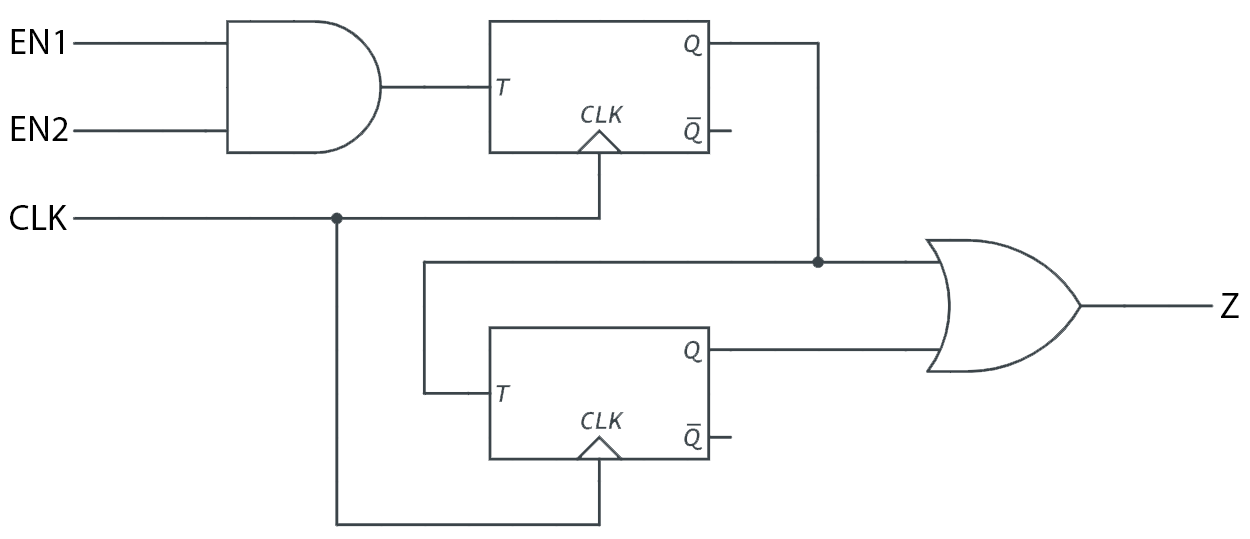
\includegraphics[width=\linewidth]{r_rtl/ex9-1.png}
	\end{minipage}

\item
\begin{minipage}[t]{1\linewidth}
	\vspace{0pt}\raggedright
	\centering
	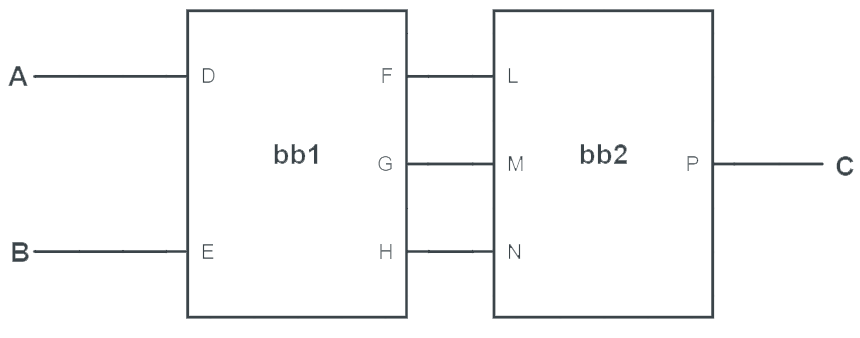
\includegraphics[width=\linewidth]{r_rtl/ex9-2.png}
\end{minipage}
\item The components for the third exercise are as follows.
\begin{lstlisting}
---------------
--- Big AND ---
---------------

LIBRARY IEEE;
USE IEEE.STD_LOGIC_1164.ALL;

ENTITY big_and IS
	PORT(
		in1,in2	:	IN	STD_LOGIC;
		out1	:	OUT	STD_LOGIC);
END big_and;

ARCHITECTURE big_and_arc OF big_and is
BEGIN
	out1	<=	in1 AND in2;
END big_and_arc;


---------------
--- Big NOT ---
---------------

LIBRARY IEEE;
USE IEEE.STD_LOGIC_1164.ALL;

ENTITY big_not IS
	PORT(
		in1		:	IN	STD_LOGIC;
		out1	:	OUT	STD_LOGIC);
END big_not;

ARCHITECTURE big_not_arc OF big_not IS
BEGIN
	out1	<=	NOT in1;
END big_not_arc;


--------------
--- Big OR ---
--------------

LIBRARY IEEE;
USE IEEE.STD_LOGIC_1164.ALL;

ENTITY big_or IS
	PORT(
		in1,in2	:	IN	STD_LOGIC;
		out1	:	OUT	STD_LOGIC);
END big_or;

ARCHITECTURE big_or_arc OF big_or IS
BEGIN
	out1	<=	in1 OR in2;
END big_or_arc;


-----------------------
--- Big 4-Input AND ---
-----------------------

LIBRARY IEEE;
USE IEEE.STD_LOGIC_1164.ALL;

ENTITY big_and4 IS
	PORT(
		in1,in2,in3,in4	:	IN	STD_LOGIC;
		out1			:	OUT	STD_LOGIC);
END big_and4;

ARCHITECTURE big_and4_arc OF big_and4 IS
BEGIN
	out1	<=	in1 AND in2 AND in3 AND in4;
END big_and4_arc;


-------------------
--- 3:8 Decoder ---
-------------------

LIBRARY IEEE;
USE IEEE.STD_LOGIC_1164.ALL;

ENTITY dec3to8 IS
	PORT(
		ins		:	IN	STD_LOGIC_VECTOR(2 DOWNTO 0);
		outs	:	OUT	STD_LOGIC_VECTOR(0 TO 8));
END dec3to8;

ARCHITECTURE dec3to8_arc OF dec3to8 IS
BEGIN
	WITH ins SELECT
		outs	<=	"10000000" WHEN "000",
					"01000000" WHEN "001",
					"00100000" WHEN "010",
					"00010000" WHEN "011",
					"00001000" WHEN "100",
					"00000100" WHEN "101",
					"00000010" WHEN "110",
					"00000001" WHEN "111",
					"00000000" WHEN OTHERS;
END dec3to8_arc;
\end{lstlisting}

a) \begin{lstlisting}
LIBRARY IEEE;
USE IEEE.STD_LOGIC_1164.ALL;

ENTITY Exercise_9_3_a IS
	PORT(
		A,B,C	:	IN	STD_LOGIC;
		F		:	OUT	STD_LOGIC);
END Exercise_9_3_a;

ARCHITECTURE Exercise_9_3_a_arc OF Exercise_9_3_a IS

	---------------
	--- Big AND ---
	---------------

	COMPONENT big_and IS
		PORT(
			in1,in2	:	IN	STD_LOGIC;
			out1	:	OUT	STD_LOGIC);
	END COMPONENT big_and;


	---------------
	--- Big NOT ---
	---------------

	COMPONENT big_not IS
		PORT(
			in1		:	IN	STD_LOGIC;
			out1	:	OUT	STD_LOGIC);
	END COMPONENT big_not;


	--------------
	--- Big OR ---
	--------------

	COMPONENT big_or IS
		PORT(
			in1,in2	:	IN	STD_LOGIC;
			out1	:	OUT	STD_LOGIC);
	END COMPONENT big_or;

	------------------------
	--- Internal Signals ---
	------------------------

	SIGNAL notA,notB,notC	:	STD_LOGIC;
	SIGNAL and1out,and2out	:	STD_LOGIC;

BEGIN

	Anot:	big_not PORT MAP(
		in1		=>	A,
		out1	=>	notA);

	Bnot:	big_not PORT MAP(
		in1		=>	B,
		out1	=>	notB);

	Cnot:	big_not PORT MAP(
		in1		=>	C,
		out1	=>	notC);

	and1:	big_and PORT MAP(
		in1		=>	A,
		in2		=>	notB,
		out1	=>	and1out);

	and2:	big_and PORT MAP(
		in1		=>	notA,
		in2		=>	notC,
		out1	=>	and2out);

	or1:	big_or PORT MAP(
		in1		=>	and1out,
		in2		=>	and2out,
		out1	=>	F);

END Exercise_9_3_a_arc;
\end{lstlisting}

b) \begin{lstlisting}
LIBRARY IEEE;
USE IEEE.STD_LOGIC_1164.ALL;

ENTITY Exercise_9_3_b IS
	PORT(
		A,B,C	:	IN	STD_LOGIC;
		F		:	OUT	STD_LOGIC;
		dec_out	:	OUT	STD_LOGIC_VECTOR(0 TO 7));
END Exercise_9_3_b;

ARCHITECTURE Exercise_9_3_b_arc OF Exercise_9_3_b IS

	-------------------
	--- 3:8 Decoder ---
	-------------------

	COMPONENT dec3to8 IS
		PORT(
			ins		:	IN	STD_LOGIC_VECTOR(2 DOWNTO 0);
			outs	:	OUT	STD_LOGIC_VECTOR(0 TO 8));
	END COMPONENT dec3to8;


	-----------------------
	--- Big 4-Input AND ---
	-----------------------

	COMPONENT big_and4 IS
		PORT(
			in1,in2,in3,in4	:	IN	STD_LOGIC;
			out1			:	OUT	STD_LOGIC);
	END COMPONENT big_and4;


	------------------------
	--- Internal Signals ---
	------------------------

	SIGNAL out0,out1,out3,out4	:	STD_LOGIC;
	SIGNAL ins					:	STD_LOGIC_VECTOR(2 DOWNTO 0);

BEGIN

	dec:	dec3to8 PORT MAP(
		ins		=>	ins,
		outs(0)	=>	out0,
		outs(1)	=>	out1,
		outs(2)	=>	dec_out(2),
		outs(3)	=>	out3,
		outs(4)	=>	out4,
		outs(5)	=>	dec_out(5),
		outs(6)	=>	dec_out(6),
		outs(7)	=>	dec_out(7));

	and4:	big_and4 PORT MAP(
		in1		=>	out0,
		in2		=>	out1,
		in3		=>	out3,
		in4		=>	out4,
		out1	=>	F);

	dec_out(0)	<=	out0;
	dec_out(1)	<=	out1;
	dec_out(3)	<=	out3;
	dec_out(4)	<=	out4;

	ins	<=	A & B & C;

END Exercise_9_3_b_arc;
\end{lstlisting}

c) \begin{lstlisting}
LIBRARY IEEE;
USE IEEE.STD_LOGIC_1164.ALL;

ENTITY Exercise_9_3_c IS
	PORT(
		A,B,C	:	IN	STD_LOGIC;
		F		:	OUT	STD_LOGIC);
END Exercise_9_3_c;

ARCHITECTURE Exercise_9_3_c_arc OF Exercise_9_3_c IS

	---------------
	--- Big AND ---
	---------------

	COMPONENT big_and IS
		PORT(
			in1,in2	:	IN	STD_LOGIC;
			out1	:	OUT	STD_LOGIC);
	END COMPONENT big_and;


	---------------
	--- Big NOT ---
	---------------

	COMPONENT big_not IS
		PORT(
			in1		:	IN	STD_LOGIC;
			out1	:	OUT	STD_LOGIC);
	END COMPONENT big_not;


	--------------
	--- Big OR ---
	--------------

	COMPONENT big_or IS
		PORT(
			in1,in2	:	IN	STD_LOGIC;
			out1	:	OUT	STD_LOGIC);
	END COMPONENT big_or;

	------------------------
	--- Internal Signals ---
	------------------------

	SIGNAL notB,notC		:	STD_LOGIC;
	SIGNAL and1out,and2out	:	STD_LOGIC;

BEGIN

	Bnot:	big_not PORT MAP(
		in1		=>	B,
		out1	=>	notB);

	Cnot:	big_not PORT MAP(
		in1		=>	C,
		out1	=>	notC);

	and1:	big_and PORT MAP(
		in1		=>	A,
		in2		=>	C,
		out1	=>	and1out);

	and2:	big_and PORT MAP(
		in1		=>	notC,
		in2		=>	notB,
		out1	=>	and2out);

	or1:	big_or PORT MAP(
		in1		=>	and1out,
		in2		=>	and2out,
		out1	=>	F);

END Exercise_9_3_c_arc;
\end{lstlisting}

d) \begin{lstlisting}
LIBRARY IEEE;
USE IEEE.STD_LOGIC_1164.ALL;

ENTITY Exercise_9_3_d IS
	PORT(
		A,B,C	:	IN	STD_LOGIC;
		F		:	OUT	STD_LOGIC);
END Exercise_9_3_d;

ARCHITECTURE Exercise_9_3_d_arc OF Exercise_9_3_d IS

	---------------
	--- Big AND ---
	---------------

	COMPONENT big_and IS
		PORT(
			in1,in2	:	IN	STD_LOGIC;
			out1	:	OUT	STD_LOGIC);
	END COMPONENT big_and;


	---------------
	--- Big NOT ---
	---------------

	COMPONENT big_not IS
		PORT(
			in1		:	IN	STD_LOGIC;
			out1	:	OUT	STD_LOGIC);
	END COMPONENT big_not;


	--------------
	--- Big OR ---
	--------------

	COMPONENT big_or IS
		PORT(
			in1,in2	:	IN	STD_LOGIC;
			out1	:	OUT	STD_LOGIC);
	END COMPONENT big_or;

	------------------------
	--- Internal Signals ---
	------------------------

	SIGNAL notA,notC		:	STD_LOGIC;
	SIGNAL and1out,and2out	:	STD_LOGIC;

BEGIN

	Anot:	big_not PORT MAP(
		in1		=>	A,
		out1	=>	notA);

	Cnot:	big_not PORT MAP(
		in1		=>	C,
		out1	=>	notC);

	and1:	big_and PORT MAP(
		in1		=>	notA,
		in2		=>	notC,
		out1	=>	and1out);

	and2:	big_and PORT MAP(
		in1		=>	A,
		in2		=>	B,
		out1	=>	and2out);

	or1:	big_or PORT MAP(
		in1		=>	and1out,
		in2		=>	and2out,
		out1	=>	F);

END Exercise_9_3_d_arc;
\end{lstlisting}
\end{enumerate}

\section*{Chapter 10}
The components used in each of the exercises are as shown below.
\begin{lstlisting}
----------------------
--- 8-bit, 2:1 Mux ---
----------------------

LIBRARY IEEE;
USE IEEE.STD_LOGIC_1164.ALL;

ENTITY mux2i1o8w IS
	PORT(
		in1,in2	:	IN	STD_LOGIC_VECTOR(7 DOWNTO 0);
		sel		:	IN	STD_LOGIC;
		out1	:	OUT	STD_LOGIC_VECTOR(7 DOWNTO 0));
END mux2i1o8w;

ARCHITECTURE mux2i1o8w OF mux2i1o8w IS
BEGIN
	WITH sel SELECT
		out1	<=	in1 WHEN '0',
					in2 WHEN '1',
					(OTHERS => '0') WHEN OTHERS;
END mux2i1o8w;

----------------------
--- 8-bit, 4:1 Mux ---
----------------------

LIBRARY IEEE;
USE IEEE.STD_LOGIC_1164.ALL;

ENTITY mux4i1o8w IS
	PORT(
		in0,in1,in2,in3	:	IN	STD_LOGIC_VECTOR(7 DOWNTO 0);
		sel				:	IN	STD_LOGIC_VECTOR(1 DOWNTO 0);
		out1			:	OUT	STD_LOGIC_VECTOR(7 DOWNTO 0));
END mux4i1o8w;

ARCHITECTURE mux4i1o8w OF mux4i1o8w IS
BEGIN
	WITH sel SELECT
		out1	<=	in0 WHEN "00",
					in1 WHEN "01",
					in2 WHEN "10",
					in3 WHEN "11",
					(OTHERS => '0') WHEN OTHERS;
END mux4i1o8w;



-------------------
--- 1:2 Decoder ---
-------------------

LIBRARY IEEE;
USE IEEE.STD_LOGIC_1164.ALL;

ENTITY decoder1to2 IS
	PORT(
		in1			:	IN	STD_LOGIC;
		out0,out1	:	OUT	STD_LOGIC);
END decoder1to2;

ARCHITECTURE dec1to2 OF decoder1to2 IS
BEGIN
	output_process:	PROCESS (in1) IS
	BEGIN
		IF (in1 = '0') THEN
			out0 <= '1';
			out1 <= '0';
		ELSIF (in1 = '1') THEN
			out0 <= '0';
			out1 <= '1';
		ELSE
			out0 <= '0';
			out1 <= '0';
		END IF;
	END PROCESS output_process;
END dec1to2;

----------------------
--- 8-bit Register ---
----------------------

LIBRARY IEEE;
USE IEEE.STD_LOGIC_1164.ALL;

ENTITY reg8 IS
	PORT(
		REG_IN	:	IN	STD_LOGIC_VECTOR(7 DOWNTO 0);
		CLK,LD	:	IN	STD_LOGIC;
		REG_OUT	:	OUT	STD_LOGIC_VECTOR(7 DOWNTO 0));
END reg8;

ARCHITECTURE reg OF reg8 IS
BEGIN
	load_process: PROCESS(CLK) IS
	BEGIN
		IF (RISING_EDGE(CLK)) THEN
			IF (LD = '1') THEN
				REG_OUT <= REG_IN;
			END IF;
		END IF;
	END PROCESS load_process;
END reg;
\end{lstlisting}
\begin{enumerate}
	\item \begin{lstlisting}
LIBRARY IEEE;
USE IEEE.STD_LOGIC_1164.ALL;

ENTITY muxreg IS
	PORT(
		A,B			:	IN	STD_LOGIC_VECTOR(7 DOWNTO 0);
		LDA,SEL,CLK	:	IN	STD_LOGIC;
		F			:	OUT	STD_LOGIC_VECTOR(7 DOWNTO 0));
END muxreg;

ARCHITECTURE muxreg_arc OF muxreg IS

	----------------------
	--- 8-bit Register ---
	----------------------

	COMPONENT reg8 IS
		PORT(
			REG_IN	:	IN	STD_LOGIC_VECTOR(7 DOWNTO 0);
			CLK,LD	:	IN	STD_LOGIC;
			REG_OUT	:	OUT	STD_LOGIC_VECTOR(7 DOWNTO 0));
	END COMPONENT reg8;

	----------------------
	--- 8-bit, 2:1 Mux ---
	----------------------

	COMPONENT mux2i1o8w IS
		PORT(
			in1,in2	:	IN	STD_LOGIC_VECTOR(7 DOWNTO 0);
			sel		:	IN	STD_LOGIC;
			out1	:	OUT	STD_LOGIC_VECTOR(7 DOWNTO 0));
	END COMPONENT mux2i1o8w;

	SIGNAL muxout	:	STD_LOGIC_VECTOR(7 DOWNTO 0);

BEGIN

	mux:	mux2i1o8w PORT MAP (
							in1		=> A,
							in2		=> B,
							sel		=> SEL,
							out1	=> muxout);

	reg:	reg8 PORT MAP (
							REG_IN	=>	muxout,
							CLK		=>	CLK,
							LD		=>	LDA,
							REG_OUT	=>	F);

END muxreg_arc;
	\end{lstlisting}

	\item \begin{lstlisting}
LIBRARY IEEE;
USE IEEE.STD_LOGIC_1164.ALL;

ENTITY muxdec2r IS
	PORT(
		X,Y,Z	:	IN	STD_LOGIC_VECTOR(7 DOWNTO 0);
		MS		:	IN	STD_LOGIC_VECTOR(1 DOWNTO 0);
		DS,CLK	:	IN	STD_LOGIC;
		RB,RA	:	OUT	STD_LOGIC_VECTOR(7 DOWNTO 0));
END muxdec2r;

ARCHITECTURE muxdec2r OF muxdec2r IS

	----------------------
	--- 8-bit, 4:1 Mux ---
	----------------------

	COMPONENT mux4i1o8w IS
		PORT(
		in0,in1,in2,in3	:	IN	STD_LOGIC_VECTOR(7 DOWNTO 0);
			sel				:	IN	STD_LOGIC_VECTOR(1 DOWNTO 0);
			out1			:	OUT	STD_LOGIC_VECTOR(7 DOWNTO 0));
	END COMPONENT mux4i1o8w;


	-------------------
	--- 1:2 Decoder ---
	-------------------

	COMPONENT decoder1to2 IS
		PORT(
			in1			:	IN	STD_LOGIC;
			out0,out1	:	OUT	STD_LOGIC);
	END COMPONENT decoder1to2;


	----------------------
	--- 8-bit Register ---
	----------------------

	COMPONENT reg8 IS
		PORT(
			REG_IN	:	IN	STD_LOGIC_VECTOR(7 DOWNTO 0);
			CLK,LD	:	IN	STD_LOGIC;
			REG_OUT	:	OUT	STD_LOGIC_VECTOR(7 DOWNTO 0));
	END COMPONENT reg8;

	SIGNAL muxout,regAout,regBout	:	STD_LOGIC_VECTOR(7 DOWNTO 0);
	SIGNAL decout0,decout1			:	STD_LOGIC;

BEGIN

	mux:	mux4i1o8w PORT MAP (
		in0		=>	regBout,
		in1		=>	Z,
		in2		=>	Y,
		in3		=>	X,
		sel		=>	MS,
		out1	=> muxout);

	dec:	decoder1to2 PORT MAP (
		in1		=>	DS,
		out0	=>	decout0,
		out1	=>	decout1);

	regA:	reg8 PORT MAP (
		REG_IN	=>	muxout,
		CLK		=>	CLK,
		LD		=>	decout0,
		REG_OUT	=>	regAout);

	regB:	reg8 PORT MAP (
		REG_IN	=>	regAout,
		CLK		=>	CLK,
		LD		=>	decout1,
		REG_OUT	=>	regBout);

	RA <= regAout;
	RB <= regBout;

END muxdec2r;
	\end{lstlisting}

	\item \begin{lstlisting}
LIBRARY IEEE;
USE IEEE.STD_LOGIC_1164.ALL;

ENTITY DualMuxDualReg IS
	PORT(
		X,Y		:	IN	STD_LOGIC_VECTOR(7 DOWNTO 0);
		LDA,LDB	:	IN	STD_LOGIC;
		S0,S1	:	IN	STD_LOGIC;
		CLK		:	IN	STD_LOGIC;
		RB		:	OUT	STD_LOGIC_VECTOR(7 DOWNTO 0));
END DualMuxDualReg;

ARCHITECTURE DualMuxDualReg_Arc OF DualMuxDualReg IS

	----------------------
	--- 8-bit Register ---
	----------------------

	COMPONENT reg8 IS
		PORT(
			REG_IN	:	IN	STD_LOGIC_VECTOR(7 DOWNTO 0);
			CLK,LD	:	IN	STD_LOGIC;
			REG_OUT	:	OUT	STD_LOGIC_VECTOR(7 DOWNTO 0));
	END COMPONENT reg8;

	-------------------------------
	--- 2-in, 1-out, 8-wide Mux ---
	-------------------------------

	COMPONENT mux2i1o8w IS
		PORT(
			in1,in2	:	IN	STD_LOGIC_VECTOR(7 DOWNTO 0);
			sel		:	IN	STD_LOGIC;
			out1	:	OUT	STD_LOGIC_VECTOR(7 DOWNTO 0));
	END COMPONENT mux2i1o8w;

	------------------------
	--- Internal Signals ---
	------------------------

	SIGNAL Mux1Out,Mux2Out	:	STD_LOGIC_VECTOR(7 DOWNTO 0);
	SIGNAL RegAOut,RegBOut	:	STD_LOGIC_VECTOR(7 DOWNTO 0);

BEGIN

	mux1:	mux2i1o8w PORT MAP(
		in1		=>	X,
		in2		=>	RegBOut,
		sel		=>	S1,
		out1	=>	Mux1Out);

	regA:	reg8 PORT MAP(
		REG_IN	=>	Mux1Out,
		CLK		=>	CLK,
		LD		=>	LDA,
		REG_OUT	=>	RegAOut);

	mux2:	mux2i1o8w PORT MAP(
		in1		=>	RegAOut,
		in2		=>	Y,
		sel		=>	S0,
		out1	=>	Mux2Out);

	regB:	reg8 PORT MAP(
		REG_IN	=>	Mux2Out,
		CLK		=>	CLK,
		LD		=>	LDB,
		REG_OUT	=>	RegBOut);

	RB	<=	RegBOut;

END DualMuxDualReg_Arc;
	\end{lstlisting}

	\item \begin{lstlisting}
LIBRARY IEEE;
USE IEEE.STD_LOGIC_1164.ALL;

ENTITY DualMuxDualReg IS
	PORT(
		LDA,LDB,S0,S1,RD,CLK	:	IN	STD_LOGIC;
		X,Y						:	IN	STD_LOGIC_VECTOR(7 DOWNTO 0);
		RA,RB					:	OUT	STD_LOGIC_VECTOR(7 DOWNTO 0));
END DualMuxDualReg;

ARCHITECTURE DualMuxDualReg_arc OF DualMuxDualReg IS

	----------------------
	--- 8-bit Register ---
	----------------------

	COMPONENT reg8 IS
		PORT(
			REG_IN	:	IN	STD_LOGIC_VECTOR(7 DOWNTO 0);
			CLK,LD	:	IN	STD_LOGIC;
			REG_OUT	:	OUT	STD_LOGIC_VECTOR(7 DOWNTO 0));
	END COMPONENT reg8;

	-------------------------------
	--- 2-in, 1-out, 8-wide Mux ---
	-------------------------------

	COMPONENT mux2i1o8w IS
		PORT(
			in1,in2	:	IN	STD_LOGIC_VECTOR(7 DOWNTO 0);
			sel		:	IN	STD_LOGIC;
			out1	:	OUT	STD_LOGIC_VECTOR(7 DOWNTO 0));
	END COMPONENT mux2i1o8w;

	------------------------
	--- Internal Signals ---
	------------------------

	SIGNAL Mux1Out,Mux2Out	:	STD_LOGIC_VECTOR(7 DOWNTO 0);
	SIGNAL RegAOut,RegBOut	:	STD_LOGIC_VECTOR(7 DOWNTO 0);
	SIGNAL And1Out,And2Out	:	STD_LOGIC;

BEGIN

	And1Out	<=	LDB AND NOT RD;
	AND2Out	<=	LDA AND RD;

	mux1:	mux2i1o8w PORT MAP(
		in1		=>	X,
		in2		=>	Y,
		sel		=>	S1,
		out1	=>	Mux1Out);

	mux2:	mux2i1o8w PORT MAP(
		in1		=>	X,
		in2		=>	RegBOut,
		sel		=>	S0,
		out1	=>	Mux2Out);

	regA:	reg8 PORT MAP(
		REG_IN	=>	Mux2Out,
		CLK		=>	CLK,
		LD		=>	And2Out,
		REG_OUT	=>	RegAOut);

	regB:	reg8 PORT MAP(
		REG_IN	=>	Mux1Out,
		CLK		=>	CLK,
		LD		=>	And1Out,
		REG_OUT	=>	RegBOut);

	RA	<=	RegAOut;
	RB	<=	RegBOut;

END DualMuxDualReg_arc;
	\end{lstlisting}

	\item \begin{lstlisting}
LIBRARY IEEE;
USE IEEE.STD_LOGIC_1164.ALL;

ENTITY DualRegDecMux IS
	PORT(
		A,B,C		:	IN	STD_LOGIC_VECTOR(7 DOWNTO 0);
		SL1,SL2,CLK	:	IN	STD_LOGIC;
		RAX,RBX		:	OUT	STD_LOGIC_VECTOR(7 DOWNTO 0));
END DualRegDecMux;

ARCHITECTURE DualRegDecMux_arc OF DualRegDecMux IS

	-------------------
	--- 1:2 Decoder ---
	-------------------

	COMPONENT decoder1to2 IS
		PORT(
			in1			:	IN	STD_LOGIC;
			out0,out1	:	OUT	STD_LOGIC);
	END COMPONENT decoder1to2;

	----------------------
	--- 8-bit Register ---
	----------------------

	COMPONENT reg8 IS
		PORT(
			REG_IN	:	IN	STD_LOGIC_VECTOR(7 DOWNTO 0);
			CLK,LD	:	IN	STD_LOGIC;
			REG_OUT	:	OUT	STD_LOGIC_VECTOR(7 DOWNTO 0));
	END COMPONENT reg8;

	-------------------------------
	--- 2-in, 1-out, 8-wide Mux ---
	-------------------------------

	COMPONENT mux2i1o8w IS
		PORT(
			in1,in2	:	IN	STD_LOGIC_VECTOR(7 DOWNTO 0);
			sel		:	IN	STD_LOGIC;
			out1	:	OUT	STD_LOGIC_VECTOR(7 DOWNTO 0));
	END COMPONENT mux2i1o8w;

	------------------------
	--- Internal Signals ---
	------------------------

	SIGNAL DecOut0,DecOut1	:	STD_LOGIC;
	SIGNAL MuxOut			:	STD_LOGIC_VECTOR(7 DOWNTO 0);

BEGIN

	dec:	decoder1to2 PORT MAP (
		in1		=>	SL1,
		out0	=>	decout0,
		out1	=>	decout1);

	mux:	mux2i1o8w PORT MAP(
		in1		=>	B,
		in2		=>	C,
		sel		=>	SL2,
		out1	=>	MuxOut);

	regA:	reg8 PORT MAP(
		REG_IN	=>	A,
		CLK		=>	CLK,
		LD		=>	DecOut1,
		REG_OUT	=>	RAX);

	regB:	reg8 PORT MAP(
		REG_IN	=>	MuxOut,
		CLK		=>	CLK,
		LD		=>	DecOut0,
		REG_OUT	=>	RBX);

END DualRegDecMux_arc;
	\end{lstlisting}

	\item \begin{lstlisting}
LIBRARY IEEE;
USE IEEE.STD_LOGIC_1164.ALL;

ENTITY DualRegMuxDec IS
	PORT(
		A,B,C			:	IN	STD_LOGIC_VECTOR(7 DOWNTO 0);
		SEL1,SEL2,CLK	:	IN	STD_LOGIC;
		RAP,RBP			:	OUT	STD_LOGIC_VECTOR(7 DOWNTO 0));
END DualRegMuxDec;

ARCHITECTURE DualRegMuxDec_arc OF DualRegMuxDec IS

	-------------------
	--- 1:2 Decoder ---
	-------------------

	COMPONENT decoder1to2 IS
		PORT(
			in1			:	IN	STD_LOGIC;
			out0,out1	:	OUT	STD_LOGIC);
	END COMPONENT decoder1to2;

	----------------------
	--- 8-bit Register ---
	----------------------

	COMPONENT reg8 IS
		PORT(
			REG_IN	:	IN	STD_LOGIC_VECTOR(7 DOWNTO 0);
			CLK,LD	:	IN	STD_LOGIC;
			REG_OUT	:	OUT	STD_LOGIC_VECTOR(7 DOWNTO 0));
	END COMPONENT reg8;

	-------------------------------
	--- 2-in, 1-out, 8-wide Mux ---
	-------------------------------

	COMPONENT mux2i1o8w IS
		PORT(
			in1,in2	:	IN	STD_LOGIC_VECTOR(7 DOWNTO 0);
			sel		:	IN	STD_LOGIC;
			out1	:	OUT	STD_LOGIC_VECTOR(7 DOWNTO 0));
	END COMPONENT mux2i1o8w;

	------------------------
	--- Internal Signals ---
	------------------------

	SIGNAL DecOut0,DecOut1	:	STD_LOGIC;
	SIGNAL MuxOut			:	STD_LOGIC_VECTOR(7 DOWNTO 0);

BEGIN

	mux:	mux2i1o8w PORT MAP(
		in1		=>	A,
		in2		=>	B,
		sel		=>	SEL1,
		out1	=>	MuxOut);

	dec:	decoder1to2 PORT MAP (
		in1		=>	SEL2,
		out0	=>	decout0,
		out1	=>	decout1);

	regA:	reg8 PORT MAP(
		REG_IN	=>	MuxOut,
		CLK		=>	CLK,
		LD		=>	DecOut1,
		REG_OUT	=>	RAP);

	regB:	reg8 PORT MAP(
		REG_IN	=>	C,
		CLK		=>	CLK,
		LD		=>	DecOut0,
		REG_OUT	=>	RBP);

END DualRegMuxDec_arc;
	\end{lstlisting}
\end{enumerate}
\resumetocwriting
